%%%%%%%%%%%%%%%%%%%%%%%%%%%%%%%%%%%%%%%%%%%%%%%%%%%%%%%%%%%%%%%%%%%%%%%%%%%%%%%%
% Template for USENIX papers.
%
% History:
%
% - TEMPLATE for Usenix papers, specifically to meet requirements of
%   USENIX '05. originally a template for producing IEEE-format
%   articles using LaTeX. written by Matthew Ward, CS Department,
%   Worcester Polytechnic Institute. adapted by David Beazley for his
%   excellent SWIG paper in Proceedings, Tcl 96. turned into a
%   smartass generic template by De Clarke, with thanks to both the
%   above pioneers. Use at your own risk. Complaints to /dev/null.
%   Make it two column with no page numbering, default is 10 point.
%
% - Munged by Fred Douglis <douglis@research.att.com> 10/97 to
%   separate the .sty file from the LaTeX source template, so that
%   people can more easily include the .sty file into an existing
%   document. Also changed to more closely follow the style guidelines
%   as represented by the Word sample file.
%
% - Note that since 2010, USENIX does not require endnotes. If you
%   want foot of page notes, don't include the endnotes package in the
%   usepackage command, below.
% - This version uses the latex2e styles, not the very ancient 2.09
%   stuff.
%
% - Updated July 2018: Text block size changed from 6.5" to 7"
%
% - Updated Dec 2018 for ATC'19:
%
%   * Revised text to pass HotCRP's auto-formatting check, with
%     hotcrp.settings.submission_form.body_font_size=10pt, and
%     hotcrp.settings.submission_form.line_height=12pt
%
%   * Switched from \endnote-s to \footnote-s to match Usenix's policy.
%
%   * \section* => \begin{abstract} ... \end{abstract}
%
%   * Make template self-contained in terms of bibtex entires, to allow
%     this file to be compiled. (And changing refs style to 'plain'.)
%
%   * Make template self-contained in terms of figures, to
%     allow this file to be compiled. 
%
%   * Added packages for hyperref, embedding fonts, and improving
%     appearance.
%   
%   * Removed outdated text.
%
%%%%%%%%%%%%%%%%%%%%%%%%%%%%%%%%%%%%%%%%%%%%%%%%%%%%%%%%%%%%%%%%%%%%%%%%%%%%%%%%

\documentclass[letterpaper,twocolumn,10pt]{article}
\usepackage{usenix2019_v3}
%\usepackage[sorting=none]{biblatex}

% to be able to draw some self-contained figs
\usepackage{tikz}
\usepackage{amsmath}

% inlined bib file
\usepackage{filecontents}
\providecommand{\shinfo}{\texttt{struct skb\_shared\_info }}
\providecommand{\page}{\texttt{struct page }}
\providecommand{\uarg}{\texttt{uarg }}
\providecommand{\kva}{kva }
\providecommand{\iova}{IOVA }
\providecommand{\mabaf}{malicious buffer }
\providecommand{\spb}{SPB\-2 }
%-------------------------------------------------------------------------------
\begin{document}
%-------------------------------------------------------------------------------

%don't want date printed
\date{}

% make title bold and 14 pt font (Latex default is non-bold, 16 pt)
\title{\Large \bf Bypassing IOMMU via the Linux Network stack}

%for single author (just remove % characters)
\author{
{\rm Markuze Alex}\\
Technion, VMware Research
\and
{\rm Gil Kupfer}\\
Technion
% copy the following lines to add more authors
\and
{\rm Nadav Amit}\\
VMware Research
\and{\rm Dan Tsafrir}\\
Technion, VMware Research
} % end author

\maketitle

%-------------------------------------------------------------------------------
\begin{abstract}
%-------------------------------------------------------------------------------
Your abstract text goes here. Just a few facts. Whet our appetites.
Not more than 200 words, if possible, and preferably closer to 150.\newline
We ignore the NDSS paper, the Linux attacks it mentiones are at best half backed, which makes our contribution valid. We will still need to address it because the whole sub-page thing; but really its the Copy paper that introduced that notion and this is how we should frame it. The steps are \#1 Write paper as if NDSS doesnt exist. \#2 Add some defensive text when \#complete
\end{abstract}


%-------------------------------------------------------------------------------
\section{Introduction}

%-------------------------------------------------------------------------------
 
%%%%%%%%%%%%%%%%%%%%%%%%%%%%%%%%%%%%%%%%%%%%%%%%%%%%%%%%%%%%%%%%%
%%%% force figure to page 3... belongs to the next section.
\begin{figure*}[t]

        \begin{lstlisting}[
        basicstyle = \small,
        %basicstyle=\ttfamily,
        columns = fixed,
        tabsize=8,
        %frame = l,
        xleftmargin=.1\textwidth,
        language = C
        ]
Start addr       |   Offset   |     End addr     |  Size   | VM area description
==================================================================================
...
ffff888000000000 | -119.5  TB | ffffc87fffffffff |   64 TB | page_offset_base
...
ffffe90000000000 |  -23    TB | ffffe9ffffffffff |    1 TB | ... unused hole
ffffea0000000000 |  -22    TB | ffffeaffffffffff |    1 TB |  vmemmap_base
...
ffffffff00000000 |   -4    GB | ffffffff7fffffff |    2 GB | ... unused hole
ffffffff80000000 |   -2    GB | ffffffff9fffffff |  512 MB | kernel text mapping
                \end{lstlisting}
        \caption{ Linux Kernel memory layout.}
        \label{fig:mem_layot}

\end{figure*}
%%%%%%%%%%%%%%%%%%%%%%%%%%%%%%%%%%%%%%%%%%%%%%%%%%%%%%%%%%%%%%%%

\section{Background}\label{sec:background}

In this section, we provide the necessary background needed to discuss DMA related attacks. First, we describe classic DMA attacks and the IOMMU protection against them. Then, we discuss well-established protection practices against privilege escalation (i.e., code injection) attacks and methods of their circumvention.

\subsection{DMA attacks}

DMA allows I/O devices, direct access to memory \cite{oC54} without CPU involvement. While DMA is essential for fast I/O, it also provides ample opportunity for unmonitored and malicious activity by DMA capable devices, i.e., DMA attacks. 

An attacker can access sensitive data and/or overwrite the OS code and data structures and even gain full control of the victim system. DMA attacks can be carried out using an external or internal DMA-capable device. 

Accessible expansion ports, e.g., FireWire or Thunderbolt, allow external devices to initiate DMA transactions merely by connecting a programmable accessory \cite{Dor04, Vol, MM, thunder}. 
Exploiting internal devices is more challenging, but enables persistent and stealthy attacks. Clearly, an internal device is simply less conspicuous than an external peripheral connected via a Thunderbolt cable.

Multiple options to gain control of an internal device are available.
A resourceful attacker can exploit firmware bugs \cite{SB12}. These can be well-known exploits, as end-users are often slow in deploying firmware updates \cite{DPVL10}, and even newly discovered zero-day vulnerabilities \cite{Ben17b}. Alternatively, certain attackers may be able to replace the device firmware altogether with a malicious one \cite{ZKB13, NL14}. It is also possible to manufacture devices that appear to be legitimate but are, in fact, malicious at the circuitry level \cite{YHD16}.

Once an attacker gained control over a DMA device connected to a victim machine, various attacks are possible, ranging from keyloggers \cite{LKV13, SB12} to full control over commodity OS and hypervisor, including Windows \cite{AD10,thunder}, Linux, OSX \cite{Fri16, thunder}, Android \cite{Ben17b}, and Xen \cite{Woj08}.

Several software tools for perpetrating DMA attacks exist, some are open source. Tools such as Volatility \cite{Vol}, Inception \cite{MM}, GoldFish \cite{GA10} and FinFireWire \cite{Fin14} can extract target machine memory and unlock victim machines by patching the OS code. These tools are reportedly used by government agencies, such as NSA.

\subsection{IOMMU}

With the lack of software protection against DMA attacks, the common practice is to restrict DMA accesses through hardware protection. The most common mechanism for this purpose is the I/O memory management unit (IOMMU). The IOMMU adds a level of indirection for DMA addresses \cite{WRC08,YZ15,SB12,MTF12}, effectively providing peripheral devices with virtual addresses termed~\iova{} (I/O virtual address). This way, the device can access only these pages that the OS has explicitly allowed. Inspired by the x86 MMU, the IOMMU uses a page table for address translation and an IO/TLB for caching recent accesses.  The page tables are managed by the OS and as with the MMU, have a page granularity. The common page size is 4\,KB, though other larger page sizes, up to GBs, also exist.

The page table also holds page access rights for each \iova. An access right can be either READ, WRITE, or BIDIRECTIONAL. Note that WRITE access does not grant a DMA device READ access, whereas BIDIRECTIONAL access is needed to both read and write from/to the page. It is also important to note that a single physical page can be mapped by multiple \iova{}s, each with a possibly different access right.

IOMMUs were not designed primarily with regard to providing security \cite{DWT79}. IOMMUs were used to allow devices that did not support vectored I/O, to access contiguous virtual memory, which may map non-contiguous physical memory \cite{Chu96, WMM97}. IOMMUs also enabled legacy devices that only supported limited address width (32-bit), to access high memory (64 bit). More recently, IOMMUs were used to assign I/O devices directly to virtual machines while maintaining their isolation properties \cite{Int16b, AMD16}. 
%Throughout this period, OS developers did not appear to consider protection against malicious devices important. To date, Windows 10 is the first Windows version that uses IOMMU for protection \cite{Mic17}.\adam{aren't these two sentences detracting from the paper? The premise is that IOMMUs are used for protection, and they contradict this premise.}
\section{Attack Mechanics}
Given that:
\begin{enumerate}
    \item IOMMU hardware is correctly implemented 
    \item IOMMU is correctly initialized on time
\end{enumerate}
One might assume that the systems are safe from DMA attacks. We contend that this is not the case. The \textit{least-privilege principle} requires that an entity such as a software module or a physical device must always have only the minimum necessary access to operate normally. In this chapter, we describe the risks caused by software when this principle is violated.
\begin{figure}[t]
    \centering
    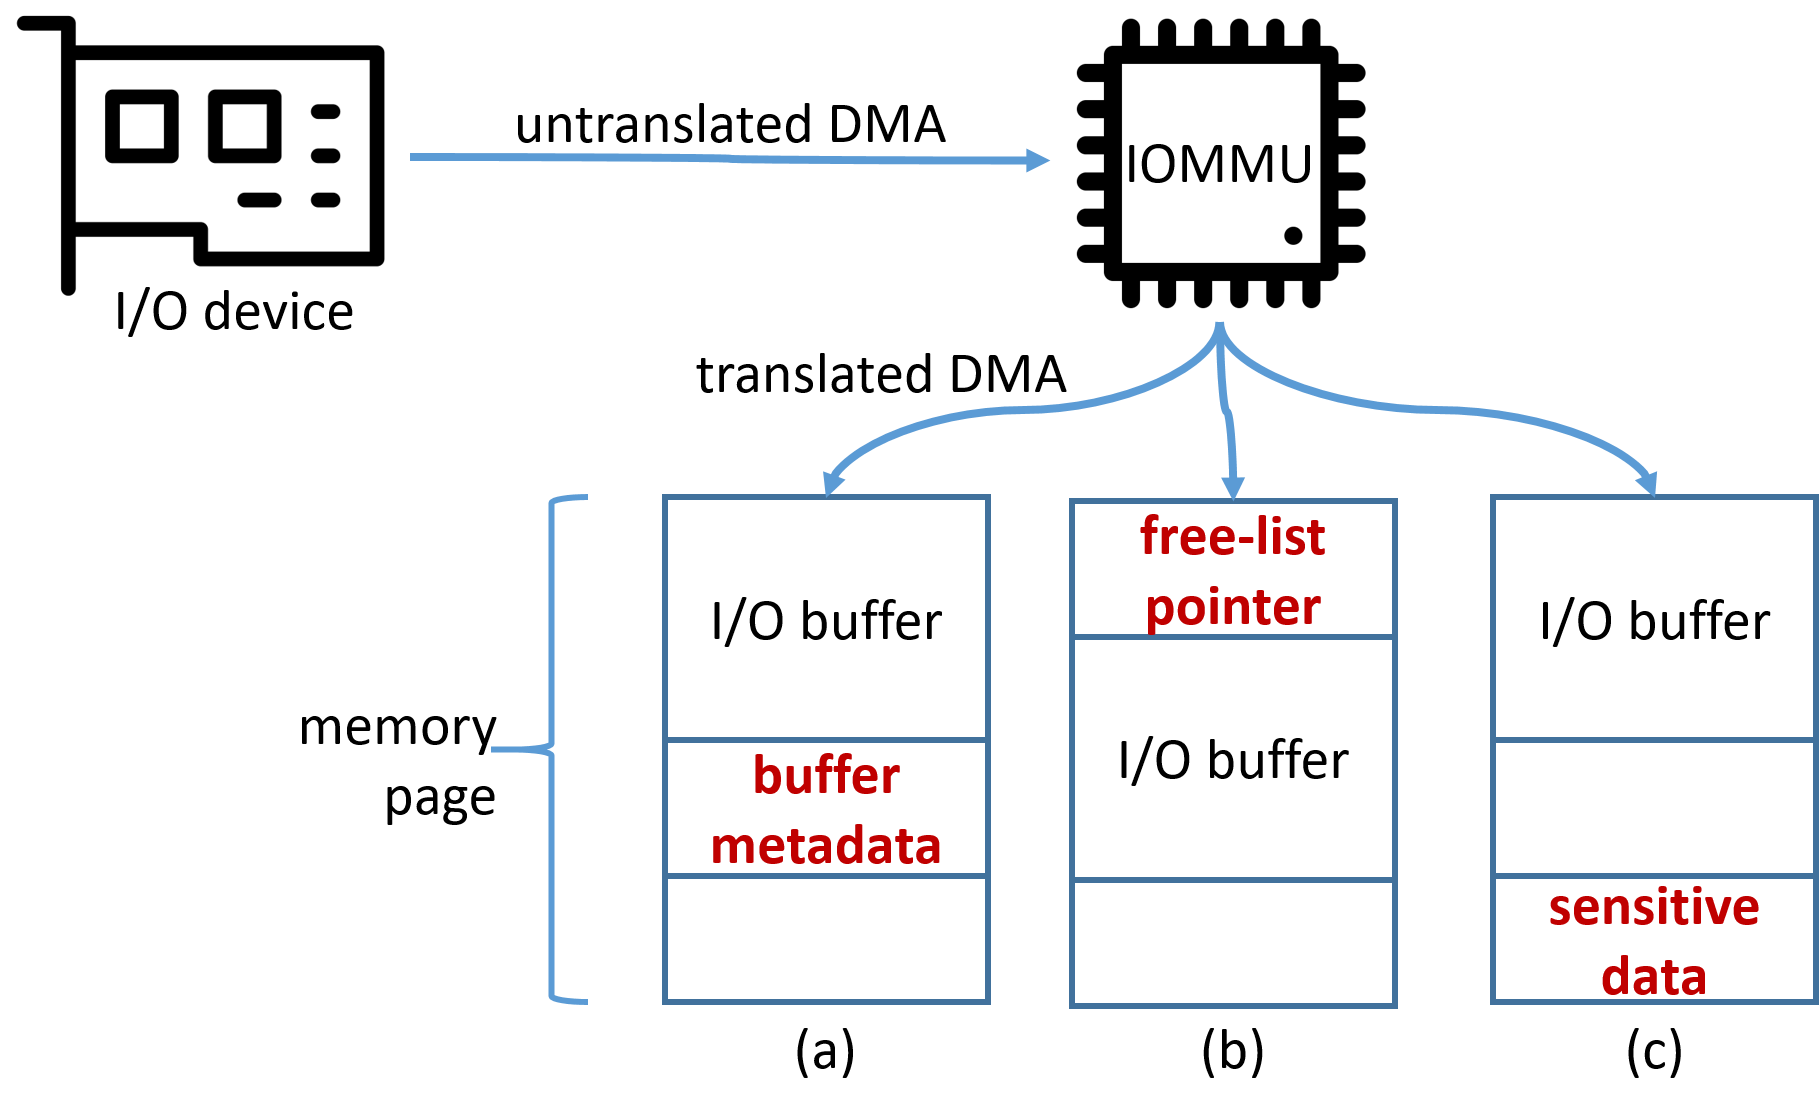
\includegraphics[width=1\columnwidth]{figs/colocation.png}
    \caption{Sub-page granularity DMA vulnerabilities when the I/O buffer resides in
a page that also holds other data: (a) I/O buffer metadata, (b) memory allocator’s
metadata such as free-list pointers and (c) randomly colocated sensitive buffers.}
    \label{fig:colocation}
\end{figure}
\subsection{Sub-Page}\label{sec:subpage}
Currently, OSs allocate I/O buffer memory using the same mechanisms they use for any memory allocation. These mechanisms, however, are oblivious to the role of the allocated memory. Consequently, I/O buffers may reside in the same page with other and potentially sensitive data. Since IOMMU protection is limited to page granularity, I/O devices that are allowed to access an I/O buffer gain access to this data as well. This behavior might compromise the system security. We classified the different types of potentially co-located data into three categories (as illustrated in Figure ~\ref{fig:colocation}: In case (a), the I/O buffer is part of a bigger data structure that also contains metadata used by the device driver. In the extreme case, this metadata might include function pointers, which enable relatively simple and robust attacks. Other fields in such data structures might be dangerous as well. In case (b), the memory allocator saves metadata, such as free-lists, with the I/O buffers, in the same page \cite{Cor07}. Manipulating these data structures may compromise the system completely \cite{ak09}. Finally, in (c), the I/O buffer and another dynamically allocated memory may reside in the same page. This common situation can easily cause data leakage, but may also be used for more sophisticated attacks. 
%We used randomly colocated pointers to break kASLR, as we discuss in Chapter 5. Why do OSs ignore the disparity between I/O buffer allocation alignment and protection granularity? One possible explanation is the benefits of dense memory allocations: lower internal memory fragmentation, which results in higher memory utilization, and lower translation lookaside buffer (TLB) pressure, which reduces the number of TLB misses. We suspect, however, that the main reason for the disparity is actually more prosaic. As IOMMUs were introduced to commodity servers relatively recently, OS developers have been reluctant to overhaul existing device drivers and change the way they allocate and manage their memory. Instead, IOMMU mapping operations were abstracted from device drivers, and implemented on top of existing DMA APIs [MHJ, The]. As a result, the memory allocation of I/O buffers has not been modified and adapted to take into consideration the IOMMU protection granularity.
\subsection{Deferred Invalidation vulnerability} 
\begin{figure*}[t]
    \centering
    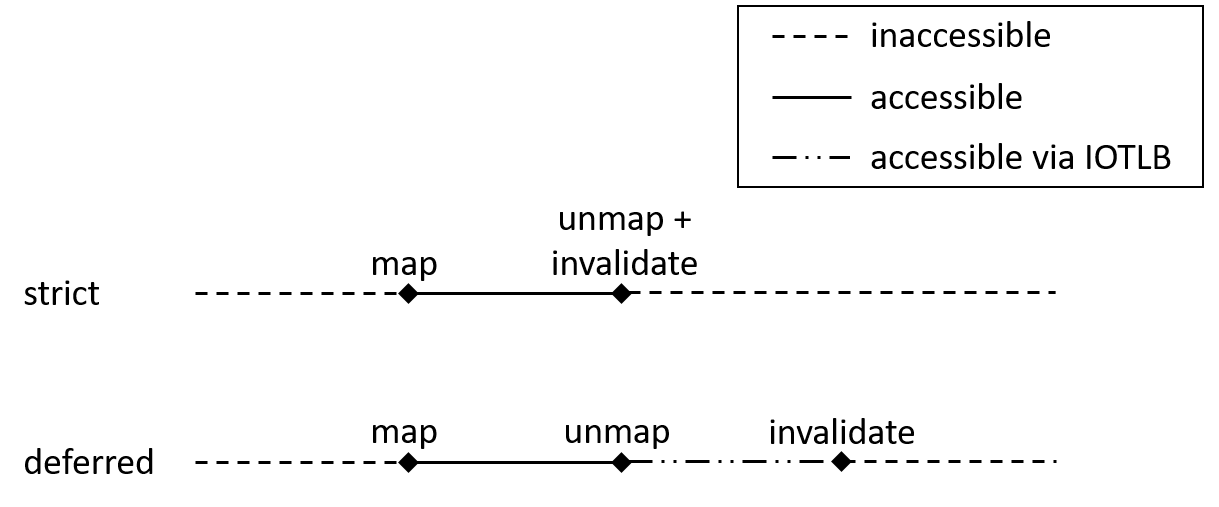
\includegraphics[width=1.3\columnwidth]{figs/deferred.png}
    \caption{Strict vs. deferred IOTLB invalidations. In deferred mode, there is a period
where the data is accessible but the mapping no longer exists.}
    \label{fig:deferred}
\end{figure*}
To translate addresses efficiently, the IOMMU caches translations in an input/output translation lookaside buffer (IOTLB). Like MMUs, IOMMUs do not maintain consistency between the IOTLB and the IOMMU page tables, which reside in memory; instead, the OS is required to restore consistency by explicitly invalidating the IOTLB. Therefore, to ensure that the IOTLB never holds stale entries, the OS must invalidate the IOTLB immediately after it removes memory mappings. Yet this scheme, called the “strict” mode in Linux, can degrade performance, as IOTLB invalidations can induce very high overhead \cite{MMT16,MSMT18,Peleg15}. In I/O intensive workloads, the number of required IOTLB invalidations can be extremely high, as IOMMU entries are unmapped following each I/O operation. Moreover, the overhead of each IOTLB invalidation can be as high as 2000 cycles \cite{ABYTS11}, considerably more than TLB invalidation, which takes roughly 100 cycles \cite{Han14}. To reduce this overhead, Linux defers TLB invalidations by default, and instead performs periodic global TLB invalidations. This “deferred” mode induces smaller performance overheads relative to the alternative “strict” mode. Nevertheless, as depicted in Figure \ref{fig:deferred}, deferring IOTLB invalidations may not prevent I/O devices from accessing unmapped pages, as the IOMMU may perform translations using stale IOTLB entries until the actual invalidation. This behavior introduces a security hazard, as the OS can reuse pages for other purposes after they are unmapped, regardless of the actual time of IOTLB invalidation. In the time window between the unmap operation and the actual invalidation, the OS may place sensitive data in the unmapped page-frame which the device may then read or modify. This time frame may be as high as 10 milliseconds when I/O traffic is low \cite{MSMT18}. In fact, this is a common scenario, as OSs prefer to reuse “hot” page-frames, recently freed, as they are likely to be already cached in the CPU caches\cite{hotcold}
. Therefore, it is possible in certain cases to predict how unmapped memory would be reused and which data it would expose.  
%As we demonstrate in Section 4.3, this behavior enables us to build robust assaults powerful enough to gain full control over a victim system.
\subsection{Threat Model}
Our attacks are built on the following assumptions:
\begin{enumerate}
    \item The actual attack is performed by a DMA-capable malicious device.
    \item There is software that violates the least-privilege principle with respect to the I/O device. The inherent vulnerabilities in the common use of the IOMMU make this a realistic assumption (§\ref{sec:sbp2_attack}). 
 \end{enumerate}
 The attacks discussed in this work are not executed by modifying the victim’s OS or drivers. We also assume that any hardware aside from the specific malicious device is working as expected, especially the DMA controller and the IOMMU itself. We also do not consider ports intended for debugging (e.g., jtag).
\subsection{Consequences}
The greatest potential consequence of our attacks is privilege escalation, which allows attackers to execute arbitrary code with kernel privileges. In all our experiments, we successfully executed code in the context of the kernel. Another potential consequence of our attacks is denial of service \cite{MMT16}. Ideally, malformed devices should not be able to crash the entire system. The IOMMU is expected to properly isolate the devices from the OS to ensure this does not happen. Bad isolation, such as colocation of different types of data in the same page, may lead to system instability. To reach the above results, the attacker must have write permissions to some memory region. When an attacker has only read permissions, the consequences may still be interesting as they may lead to data leakage\cite{thunder}. The kernel often keeps sensitive data such as encryption keys and passwords as plain-text in memory. Attackers may use incorrect read permissions to leak this sensitive data.
\section{OS Defences}
In this section we discuss the common mechanisms used to mitigate code injection attacks. Subverting these countermeasures is essential to the success of any DMA attack.

\subsection{NX-BIT}\label{sec:nx-bit}
When exploiting a sub-page vulnerability (section \ref{sec:subpage}) a peripheral device has access with read/write permissions to memory buffers it shouldn't. Gaining write access to a function pointer can allow the attacker to inject malicious code. DMA capable devices, usually get access to pages with data, rather than code. Modern OSs make use of hardware support, namely the No-eXecute bit, to prevent running code from data pages. The bit for each page is defined in MMU’s page tables. Whenever the CPU tries to fetch code from memory, this bit is checked. If it is set, instead of running the code, the CPU will raise an exception to the OS, notifying it that someone is trying to break into the system. This method is known under the names NX\-bit, W xor X (Write xor eXecute) and DEP and it is intended to prevent code injection attacks.\newline
Return Oriented Programming (ROP) Return Oriented Programming (ROP) is a common method used by malware to bypass DEP defenses \cite{RBSS12}. ROP takes advantage of the fact that the CPU stack pointer may point to any data page. To set up an attack from a data page, the attacker builds a stack filled with required data and pointers to special locations in the code section (aka ROP gadgets) in it. Each gadget is a short piece of code—usually one or two commands, and a return command. When the CPU executes a return command, the next address to fetch code from is taken from the stack. In the stack the next address points to another gadget and so on. By carefully selecting these gadgets, an attacker can execute any payload. For a ROP attack to succeed, an attacker needs the stack pointer to point at the poisoned stack. We turn to Jump Oriented Programming ;(JOP) is a similar technique that uses jumps instead of returns and, therefore, does not need the stack\cite{BJFL11}.We use JOP gadgets that direct the stack pointer to the desired page, to jump-start the ROP attack. 

%#define __PAGE_OFFSET           page_offset_base
%#define PAGE_OFFSET ((unsigned long )__PAGE_OFFSET)
%#define VMEMMAP_START          vmemmap_base
%#define vmemmap ((struct page *)VMEMMAP_START)

\begin{figure*}[t]
                \begin{lstlisting}[
        %basicstyle = \scriptsize,
        columns = flexible,
        tabsize=8,
        %frame = l,
        language = C
        ]
        
#define __va(x) ((void *)((unsigned long)(x) - PAGE_OFFSET))
#define __pa(x) ((unsigned long)(x) + PAGE_OFFSET)

#define virt_to_pfn(kaddr)      (__pa(kaddr) >> PAGE_SHIFT)
#define pfn_to_virt(pfn)        __va((pfn) << PAGE_SHIFT)

        /* memmap is virtually contiguous.  */
#define __pfn_to_page(pfn)      (vmemmap + (pfn))  
#define __page_to_pfn(page)     (unsigned long)((page) - vmemmap)
                \end{lstlisting}
        \caption{ Linux Macros for transition between KVA, PFN and \page.
                }
        \label{fig:mem_model}
\end{figure*}
\subsection{KASLR}\label{sec:kaslr}
Address Space Layout Randomization (ASLR) is a common mechanism for mitigating code-execution attacks in the context of user-level processes. To inject code into a process, the attacker must know the memory layout. For example, the address of the code section is required for finding ROP gadgets \ref{sec:nx-bit}. Systems that support ASLR randomize the memory layout for each process on every execution. In this way, regular attacks, which are built for a specific layout, fail. Similarly, KASLR \cite{kalsr} randomizes the memory layout of the kernel. The Linux kernel has a predetermined virtual memory layout\footnote{\url{https://elixir.bootlin.com/linux/latest/source/Documentation/x86/x86_64/mm.rst}} KASLR treats the entire kernel text mapping as a single region, randomizing only its base address. Linux Kernel text addresses are always in the range [0xffffffff80000000,0xffffffffa0000000) and, therefore are very easy to detect. KASLR kernel text is aligned to 2MB boarders\footnote{This is the result of page table restrictions and unlikely to change}, which means that the lowest 21 bits remain unchanged with KASLR. Hence, knowing even one address of a known element is enough to deduce the base address and break KASLR. Once the base address is known, the attacker can use it to create a ROP stack. Malicious devices can scan pages mapped for reading, looking for kernel pointers colocated with their buffers. Once such a pointer is identified, all that remains is to reduce the offset of the symbol in the binary from the pointer to get the base address. We found that there is a symbol visible to both FireWire and NICs in all Linux versions we have tested, making it suitable for breaking kASLR. Starting from version 2.6.24, Linux supports network namespaces for isolating different instances of network use. Every network object (and sockets, in particular) has a pointer to its namespace object. Moreover, at least one namespace is always defined by the global object \texttt{init\_net}. Since TX packets have varying sizes, NICs can see all kinds of dynamically allocated objects, including sockets. In addition, socket objects are about the same size as sbp2 management orb, making them allocated from the same pages. Hence, both of them can see socket objects and, thus also the address of \texttt{init\_net}. Using this pointer, the attacker can deduce the base address and complete the ROP attack. \newline Starting from Linux 4.8, the direct mapping base, and virtual memory map are also randomized, each regions base pointer is randomized at a 1GB alignment; which means that the lover 30 bits are unmodified and can leak both the PFN numbers and the randomized offset. This alignment is also due to page table considerations (page upper table(PUD) has a 30bit shift). We will need to know both offsets for the attacks in sections \ref{sec:linux_net}. Once, the random offsets \textit{PAGE\_OFFSET} and \textit{vmemmap} for direct mapping base and virtual memory map, are known; we can transition between a \kva its PFN and its \page address. The translation macros are shown in Fig \ref{fig:mem_model}.  

\begin{comment}
\textcolor{olive}{
\subsection{breaking kaslr with leaked pointers}
Please make prev section coherent...
\begin{itemize}
    \item PUD alignment
    \item page\_offset\_base
    \item vmemmap\_base
    \item kernel text offset
\end{itemize}}
\end{comment}

\section{\simple{} Attacks}\label{sec:attack_setup}

In this section, we discuss \simple{} attacks, i.e., exploits in which the trifecta appears within a single page.
We find several such potential \simple{} exploits in the Linux kernel. We detail such an example in the FireWire driver, as this is the hardware we have in our setup. 



\subsection{Attack setup}
In our attacks, we use a Dell PowerEdge R610 server, an Intel x86 machine with Ubuntu 18.04 (kernel version 4.15), as our victim machine. The server is equipped with Intel VT-d IOMMU a Broadcom NetXtreme II BCM5709 Gigabit Ethernet NIC, a Mellanox Technologies ConnectX-4 Ethernet NIC and VIA Technologies, Inc. VT6315 Series Firewire Controller. An identical machine connected to the victim with a FireWire cable acting as the attacker. 

We create a malicious FireWire device by modifying the Linux-IO Target (LIO) subsystem on the attacker machine. The LIO subsystem supports hard disk emulation for remote computers via the \spb{} protocol; and, as such, is a suitable platform to execute such attacks. 

We implement multiple attacks against the Linux kernel network stack. In order to demonstrate an attack by a malicious NIC, we use a FireWire device similarly to \cite{SLND10}. To emulate an attack by a malicious NIC using a FireWire device, we create an \iova{} page table sharing between the FireWire and the actual NIC. A minor patch is needed for the victim OS to facilitate this emulation. This way, the attacker machine can access the same pages as the Broadcom NIC, which allows us to execute an attack using a programmable interface, emulating a malicious NIC.

\subsection{FireWire Background}

The FireWire protocol is a serial replacement for the parallel SCSI bus, which provides connectivity for digital audio and video equipment. The SBP-2 (serial bus protocol $\#2$) enables the use of SCSI devices over Firewire. 

While Firewire is a somewhat outdated physical connector, rarely in use for modern systems, some cables allow seamless conversion between Firewire and Thunderbolt. This allows for Firewire use in modern setups.

A SCSI connection consists of two endpoints: an initiator' (i.e., OS), which initiates SCSI session, and a target (i.e., a disk), which holds for the initiator's commands and provides the required I/O data transfers. 

Linux has a Linux-IO (LIO) module, which allows for a Linux machine to act as a SCSI target. One can boot the machine in \emph{target disk mode}, such that it acts as a disk (i.e., SCSI target) when connected to another computer. When the connection is via FireWire, the SPB2 protocol is used.

\subsection{Linux FireWire Exploit} \label{sec:sbp2_attack}
\begin{figure}
    \centering
    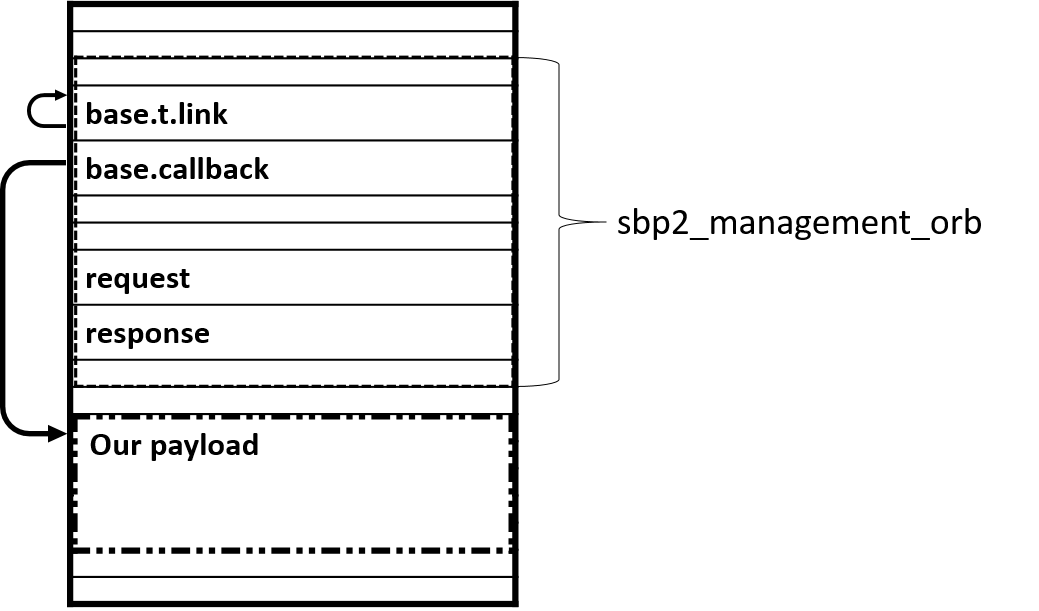
\includegraphics[width=1\linewidth]{figs/sbp.png}
    \caption{\texttt{spb2\_management\_orb} struct with fields relevant to the DMA attack.}
    \label{fig:orb}
\end{figure}

The Linux FireWire driver has a type (a) (Fig. \ref{fig:colocation} (a)) sub-page vulnerability. Both the device metadata and the I/O buffers for the \spb{} protocol implemented by the spb2 driver are contained inside the \texttt{spb2\_management\_orb} struct (Fig. \ref{fig:orb}). This provides the attacker with both \means{} and \oportunity{}.

To enable communication between the initiator and the target, the spb2 driver maps the request and response fields. As a result, the whole 4~KB page, that contains the \texttt{spb2\_management\_orb} struct is accessible with both READ and WRITE to the device. Read access is available via the \iova{} created when the \emph{request} was mapped. Write access is available via the \iova{} created when the \emph{response} was mapped. Consequently, the device can read and manipulate both the request and response fields as well as the metadata. 

Additionally, the \texttt{spb2\_management\_orb} struct contains a callback function \texttt{base.callback} which provides the \oportunity{}. Generally, to preserve normal device behavior, the original callback should also be called before or after the malicious code. However, in our experiments, we have found that ignoring the original callback has no ill side effects. 

The \texttt{spb2\_management\_orb} struct also holds its own address in the \texttt{base.t.link} field, and thus provides the attacker with \means{}. At this point, the attacker can create a \mabaf{} on the same page and complete the MMO trifecta. 

The code of the \mabaf{} appears in Appendix \ref{apx:shellcode}. It is also important to note that in this attack KASLR was irrelevant, as the critical \kva{} appeared in full, inside the readable page.

\smallskip
\noindent \textbf{Remark 1.} To date (kernel 5.3), the \texttt{spb2\_management\_orb} struct has not changed.

\smallskip
\noindent \textbf{Remark 2.} Additional such exploits, also appear in these drivers(a partial list) : nvme\_fc driver, and others...\footnote{\textcolor{red}{Find more}},
The difference in detailing each such exploit would extend only to the structure names. \SV{dempstrate the tool.. say the tool found it and give examples...}
\section{Compound DMA attacks}\label{sec:linux_net}
\begin{figure}
    \centering
    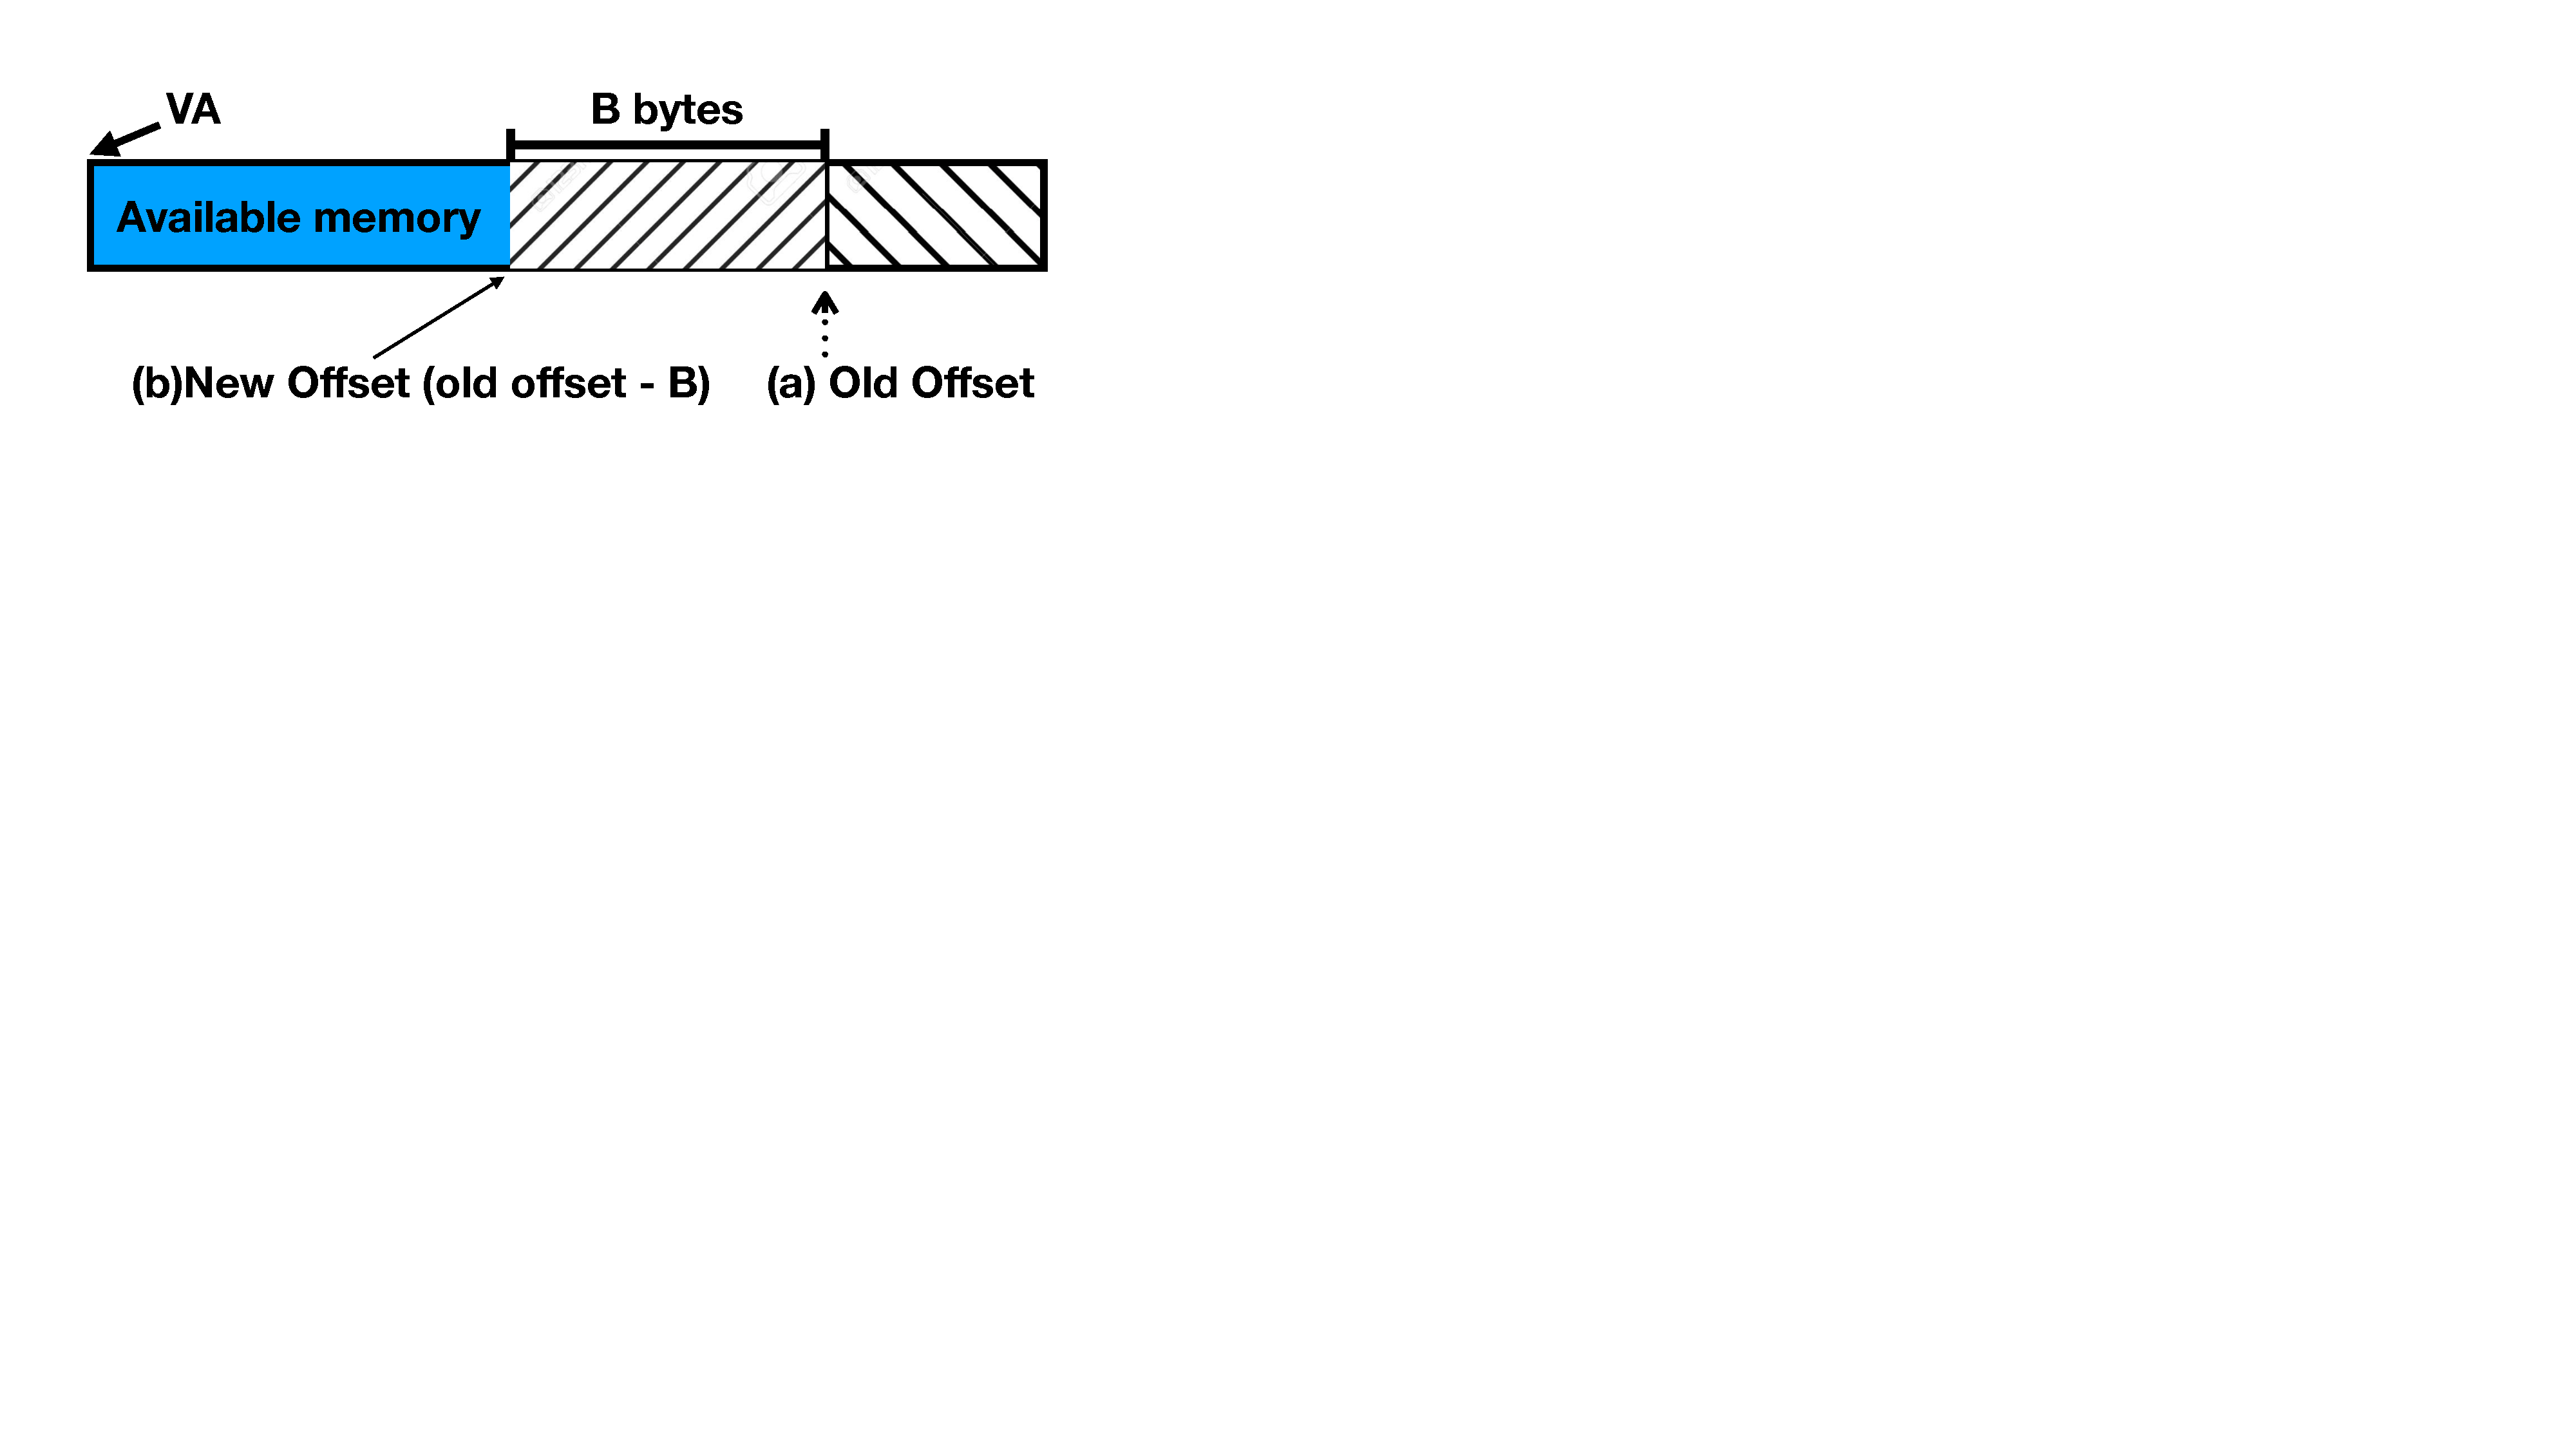
\includegraphics[width=1\linewidth]{figs/page_frag.pdf}
    \caption{Allocation of B bytes from page\_frag}
    \label{fig:page_frags}
\end{figure}

So far, we have discussed how a malicious device can take over a machine by exploiting type (a) sub page vulnerability of the FireWire driver. In this section we explore new attacks on the Linux network stack; where \means{} and \oportunity{} 
are initially missing but are attainable via compound steps, leaving room to dangerous privilege escalations attacks.

\subsection{\shinfo}
\begin{figure}[t]
    \centering
    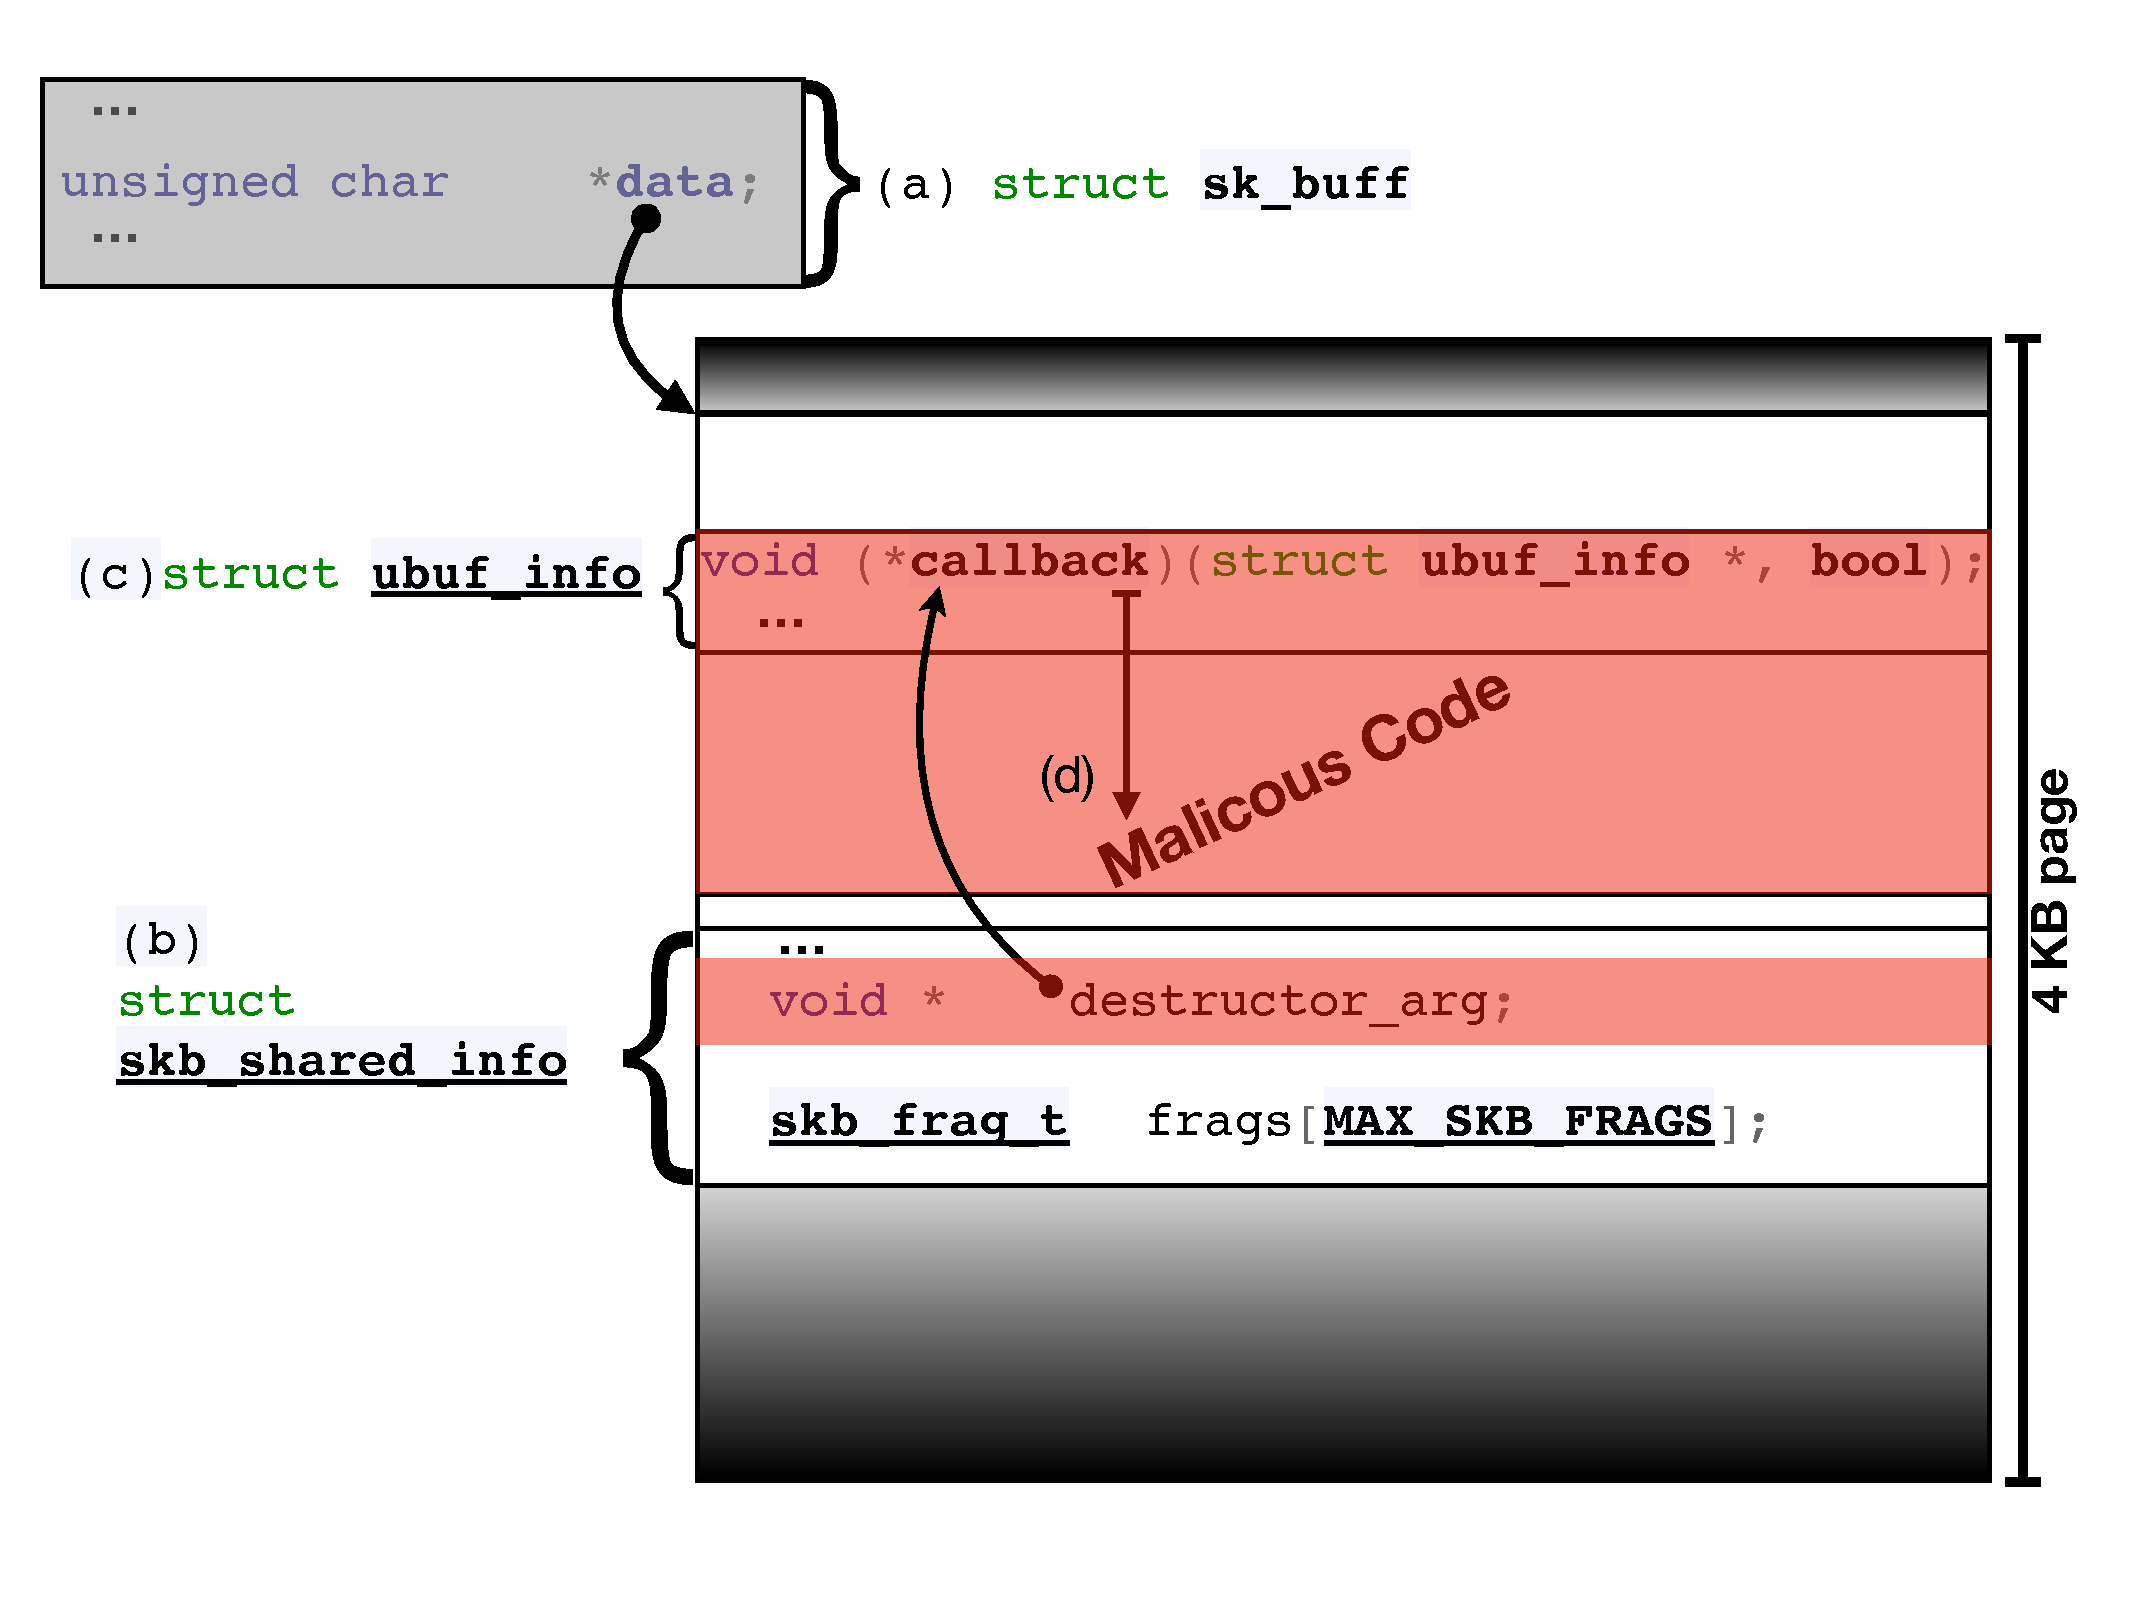
\includegraphics[width=\linewidth]{figs/ubuf.pdf}
    \caption{Using \shinfo{} to execute arbitrary code in kernel context.}
    \label{fig:sh_info}
\end{figure}

Struct \skb{} is a common data structure, used by the Linux network stack, to hold information representing a network packet. Struct \skb{} holds the metadata of a network packet (e.g., its size, associated socket). One of these fields is a pointer to a data buffer. The data is allocated separately, and thus, does not share a page with its \skb{} (Fig. \ref{fig:sh_info}). 

This separation means that \skb{} is \emph{never} (intentionally) mapped to the device. Indeed, it is a common belief, pointed out in literature \cite{thunder}, that the Linux network stack is not susceptible to DMA attacks via the \texttt{data} pointer. In this work, we show that this belief is misplaced.

The Linux network stack supports packet cloning by merely copying \skb{} metadata. This includes the \texttt{data} pointer. That is, the resulting \skb{} and the original one share the data buffer \cite{drivers2005linux}. Note that the data buffer of the \skb{} is the \emph{linear} part of the payload but \skb{} also supports \emph{non-linear} buffers, ferrying payloads in page fragments (i.e., buffers described by their \page{}, length and offset). 

To support these non-linear buffers, the \shinfo{} metadata structure is used.
Struct \shinfo{}, in contrast to \skb{}, is always allocated as part of the data buffer. Therefore it is always mapped to the device. \shinfo is unwittingly mapped with the permissions of the packet, i.e., WRITE for RX packets, READ for TX packets, and in some cases, such as XDP/XSK \cite{xdp} with BIDIRECTIONAL.

Consequentially, \shinfo{} is the potential \oportunity{} the malicious device has been looking for. The sub page vulnerability created by \shinfo{}, represents a type (b) vulnerability (Fig. \ref{fig:colocation} (b)), as this is innate to Linux networking rather than a driver security bug. 

Fig. \ref{fig:sh_info} depicts how a malicious device can mount an attack using \shinfo{} in four steps:
\begin{enumerate}[label=(\alph*)]
    \item An RX \skb{} and its data buffer are allocated. The data buffer is mapped for the NIC with WRITE access (the WRITE access is to the whole 4~KB page). 
    \item \texttt{destructor\_arg} field in \shinfo{} is overwritten to point within the mapped page. Now, the \texttt{destructor\_arg} is pointing to struct \uarg{} which is created by the NIC.
    \item \uarg{} has a callback pointer that is now pointing to the malicious code that resides on the same page. In the case of NX-bit, it is a poisoned ROP stack.
    \item when the \skb{} is released, the callback is invoked.
\end{enumerate}
To expand this scenario into a complete attack, the attacker must complete the MMO trifecta. That is, both \means{} and \oportunity{} are required. \textcolor{olive}{In the next subsection, we demonstrate how an attacker can leverage the standard OS behavior to find the missing attributes.}

\subsection{Hacking~\oportunity{}}\label{sec:shinfo}

\begin{figure}[t]
    \centering
    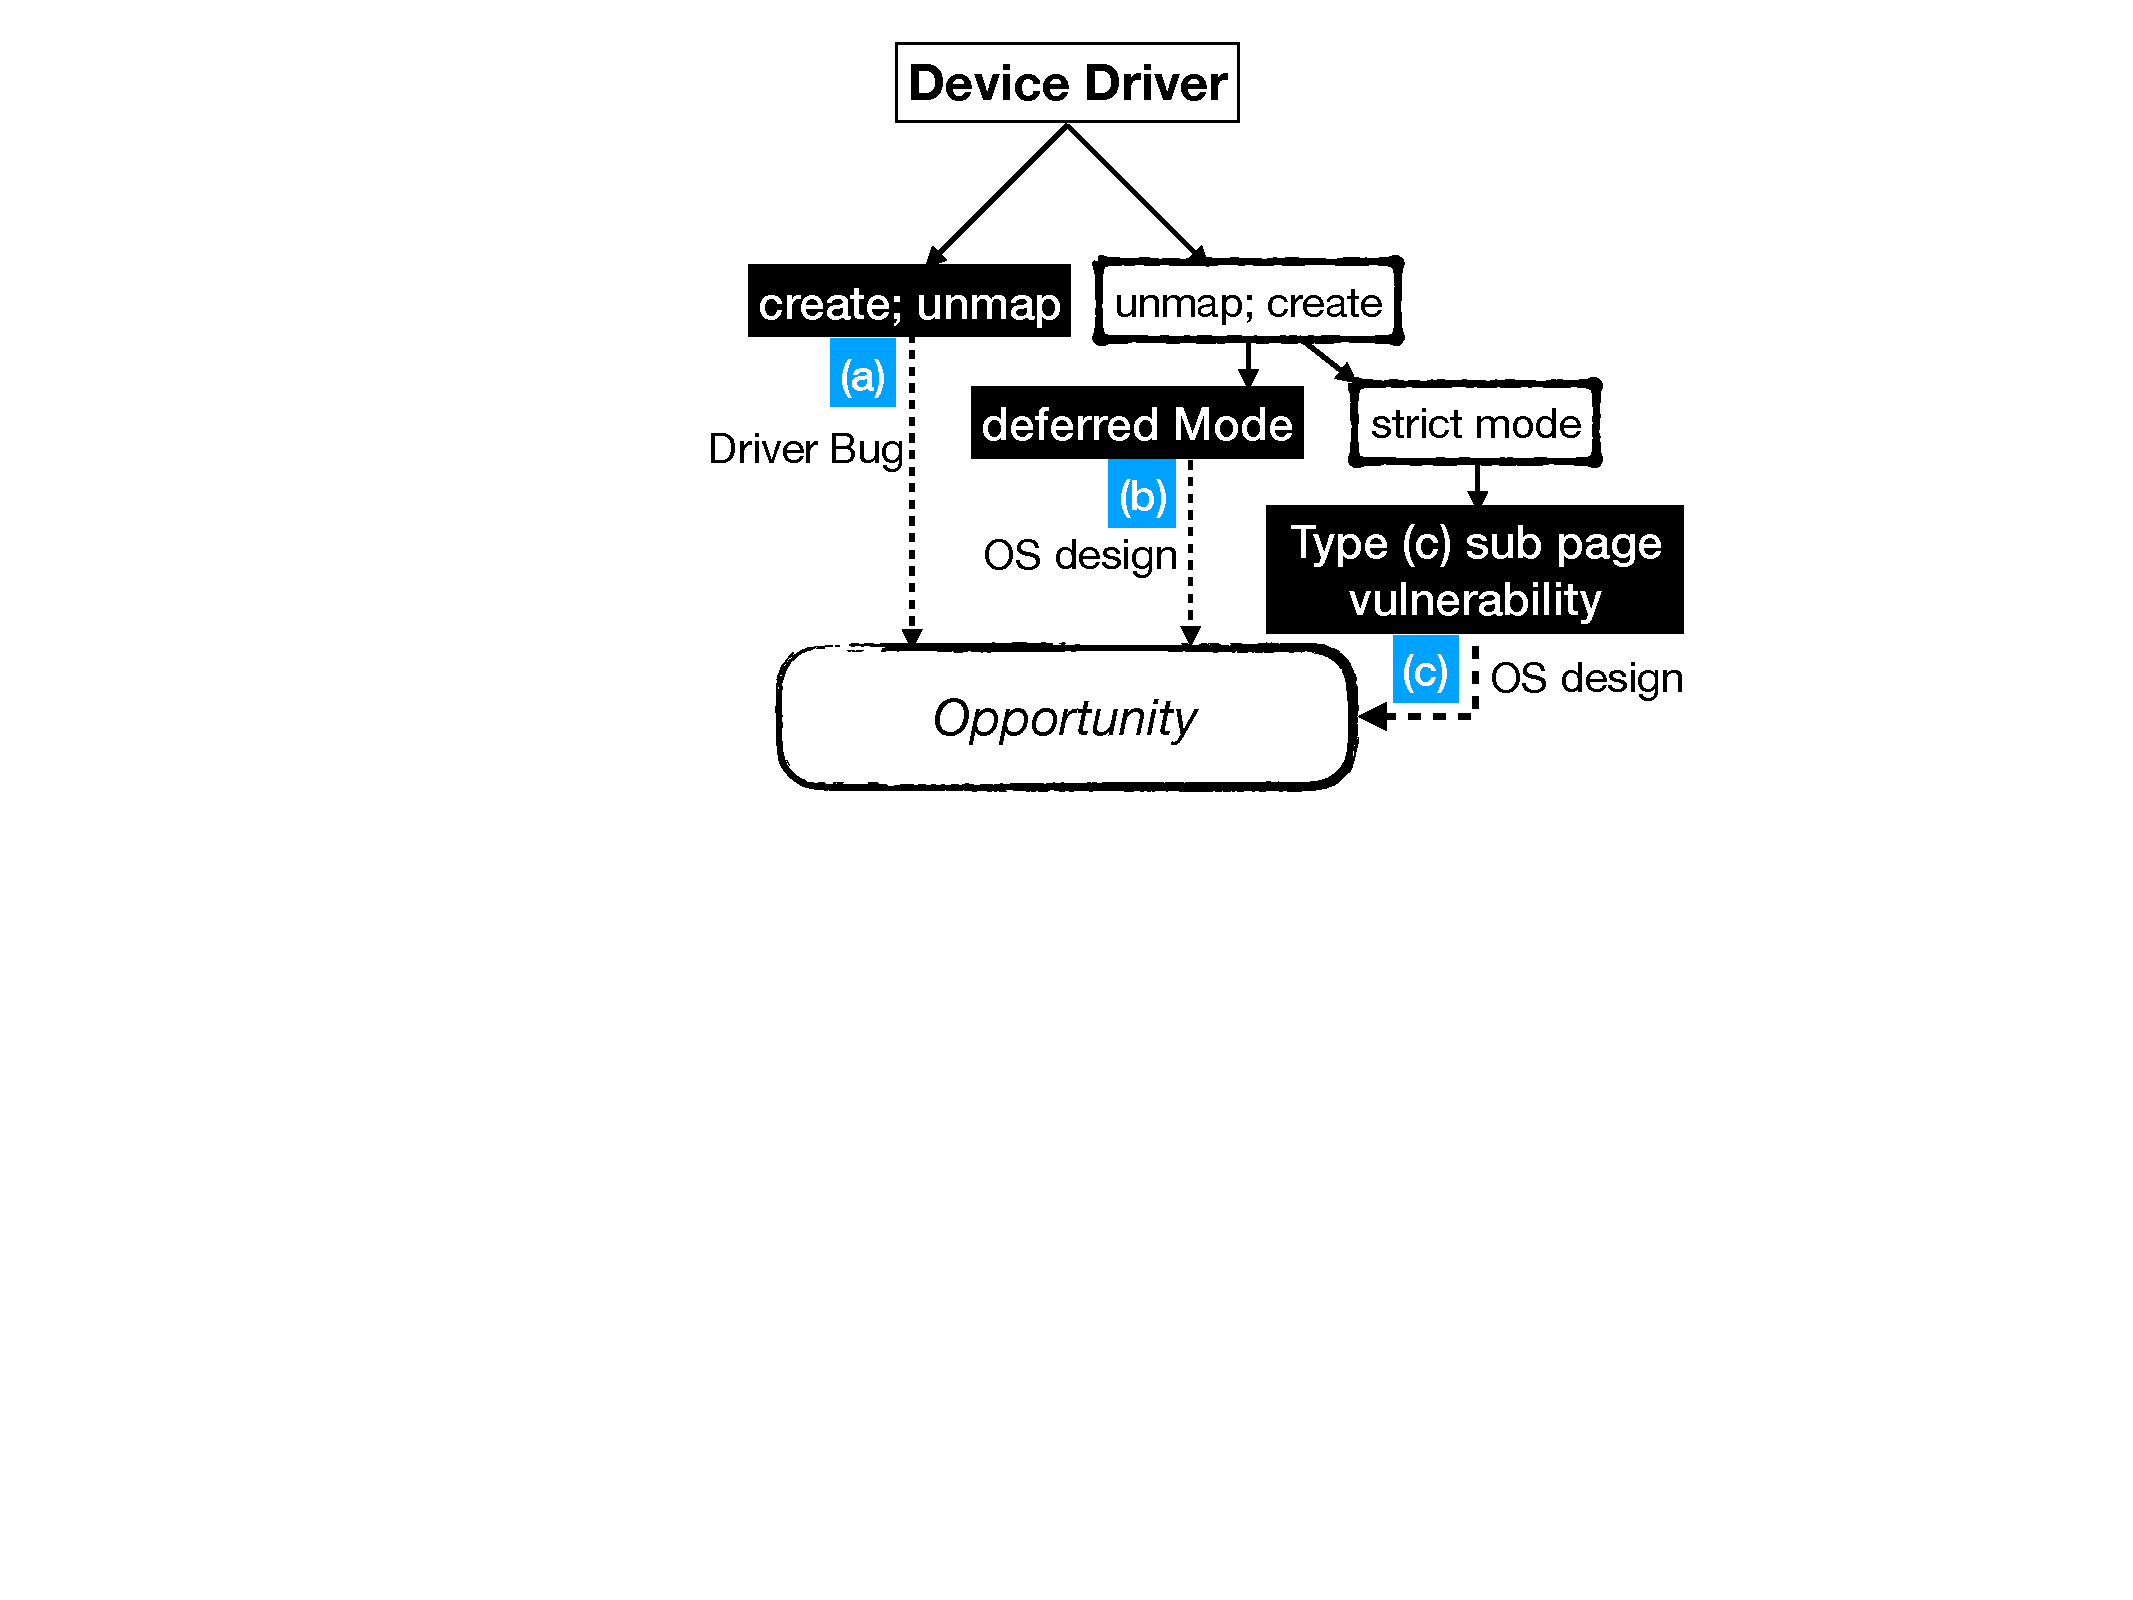
\includegraphics[width=\linewidth]{figs/road_to_op.pdf}
    \caption{Different ways to obtain \oportunity.}
    \label{fig:road_to_op}
\end{figure}

As depicted in Fig. \ref{fig:road_to_op}, we now details different ways ((a), (b) and (c)) in which a malicious device obtains \oportunity{}.

\begin{enumerate}[label=(\alph*)]

\item Presumably, a correct use of the DMA API should thwart the attack outlined in the previous section (Fig. \ref{fig:sh_info}). Namely, unmapping the buffer and only then initializing \shinfo{} should allow the CPU to undo any malicious changes the NIC may have perpetrated. 
As it turns out, prevalent device drivers (Appendix \ref{apndx:wrong_order}) first create an \skb{} and only then unmap the buffer. This order of execution allows the \emph{device} to undo legitimate changes to \shinfo{} by the CPU. 

\item Nevertheless, even when the order is correct, i.e., the unmapping of the buffer occurs before the creation of the \skb{}, still \shinfo{} is not safe from later modifications. As the default IOMMU mode in Linux is \emph{deferred} protection (Sec. \ref{sec:deferred}), the umap order is made irrelevant. That is, even though the unmap function is invoked in the correct order, the device can still corrupt \shinfo{} due to the IOTLB. Namely, the device can control which \iova{} are cached in the IOTLB by accessing only the addresses it needs cached. 

\item In response, a security-conscious admin may change the default setting to \emph{strict} mode, where the IOTLB is flushed on every unmap. However, this both severely degrades networking performance \cite{MMT16,MSMT18}, and does not alleviate the security threats on the system. Presumably, with \emph{strict} mode enabled, the \iova{} the NIC used to access that \shinfo{} is no longer valid, which initially sounds promising. The problem is that the device, in many cases, will still have legitimate WRITE access to the physical page of the \shinfo. The vulnerability stems from the way \data{} is allocated. An RX \skb{} is almost exclusively allocated via an API (e.g., \texttt{napi\_alloc\_skb} or \texttt{netdev\_alloc\_skb}) that creates a type (c) sub page vulnerability (Fig. \ref{fig:colocation} (c)). The device can use the \iova{} of a co-located buffer to access the \shinfo{} it requires. Particularly, the buffers of the driver RX ring are allocated sequentially, resulting in pairs of successive RX descriptors that map the same page. Obviously, this holds as long as the buffer sizes are smaller than 4 KB. This is a reasonable assumption since the default MTU size is 1500~B. These allocation functions, use a \texttt{page\_frag} mechanism to allocate the \data{} buffers, which in turn contain \shinfo. The \texttt{page\_frag} is an efficient method for allocating small buffers, often used by the Linux network stack. A \texttt{page\_frag} is initialized by allocating a contiguous memory region (usually 32 KB), setting a \textit{va} pointer to the beginning of the region and \texttt{offset} to the end. An allocation request for \texttt{B} bytes subtracts \texttt{B} bytes from the \texttt{offset} pointer and returns the new value of \texttt{offset}\footnote{In multicore environments, the \texttt{page\_frag} uses a different buffer for each CPU and each CPU has a single RX ring. As a result, each RX ring is served by its own (per-CPU) contiguous buffer.} (Fig. \ref{fig:page_frags}). This mechanism for memory allocation is efficient, but results in consecutive \data{} buffers sharing memory pages. Due to this type (c) sub page vulnerability, the NIC does not require the invalidated \iova{} to modify the \shinfo; instead, it can use the \iova{} for the next data buffer. Note that the lower 12 bits (the offset on the page) of the \iova{} are identical to the corresponding \kva{} bits. As illustrated in Fig. \ref{fig:sh_info}, the \oportunity{} obtained is via the next buffer (i.e., the striped area at the end of the page).
\end{enumerate}

\textcolor{olive}{
The drivers on our setup, namely bnx2 and mlx5\_core are both vulnerable. The bnx2 driver uses the correct unmapping order, and uses kmalloc to allocate its RX buffers, instead of the dedicated API functions (e.g., \texttt{napi\_alloc\_skb} or \texttt{netdev\_alloc\_skb}), but due to \emph{deferred} mode, \shinfo{} is still vulnerable to modifications.
The mlx5\_core driver, avoids unmapping the RX buffers altogether, in kernel 5.0, the driver uses a \texttt{pool\_page} mechanism\cite{page_pool} and in kernel 4.15, the driver uses an ad-hoc mechanism, to achieve the same goal as \texttt{pool\_page}. These, design choices, in both cases leave \shinfo{} vulnerable, both in \emph{deferred} and \emph{strict} modes.  
The discrepancy in driver behavior, is due to the fact that bnx2 is a driver for a 1 GBE NIC; where as, mlx5\_core is a 50 GBE\footnote{\textcolor{red}{Ours is an x8 model rather than the x16, that can reach 100GB/s.}}, and uses more efficient APIs to maximise performance.}



\smallskip
Interestingly, as it stands today, it seems that the only way to secure \shinfo{} is to never map it. 


\smallskip
\textcolor{olive}{From this point on, we assume that the attacker has unimpeded access to \oportunity{}. In the next subsections, we demonstrate various compound DMA attacks where an attacker can exploit OS behaviour to gain \means{} and \motivation{} completing the trifecta.}

\subsection{Ring Flod}\label{sec:ringflod}

A malicious device can generate a poisoned ROP stack on each RX buffer and gain \motivation{}. At this point, the device still cannot execute a successful code injection attack; the device is lacking \means{}. 

Due to the IOMMU, the device has all the \iova{} for the RX buffers, but not the \kva{}. In this attack we take advantage of the fact that the boot process is \emph{deterministic}. Each reboot, the same set of commands is executed in the same order initiating the same kernel modules and starting the same processes. While the actual pages each module gets vary in a multi-core machine due to timing issues, the drift is not expected to be too large.

We evaluate this assumption also on a DELL 730 server equipped with a ConnectX-4 NIC, running 256 reboots on Ubuntu 18.04 with kernel 5.0. 
\footnote{\textcolor{red}{Please generate table of RingFlod Results}}

We find that many of the PFNs repeat in more than 50\% percent of reboots. \footnote{\textcolor{magenta}{Need to see If we can improve this number}} Thus an adversary with knowledge about the physical setup can guess with a high probability a valid \kva{} for one of the RX pages. Now with a valid \kva{} for a \mabaf{},  i.e., \means{} and \motivation{}, the trifecta is complete and the attacker is able to execute the attack as shown in Fig. \ref{fig:sh_info} (in this case the \texttt{destructor\_arg} will most likely indicate a different page, but other that the attack scenario is unchanged).

The success probability of this attack depends on the driver version and NIC capabilities. For example ,some NICs have a HW LRO capability; where a NIC can aggregate multiple TCP packets into a single TCP packet, larger than MTU \cite{mlx5_lro}(e.g., bnx2x, mlx5\_core). On drivers configured with these options each RX buffer is 64KB regardless of MTU. As a result, these drivers have a much larger memory footprint\cite{MSMT18} and are much easier to target with a RingFlod attack.

\begin{figure*}[t]
    \centering
    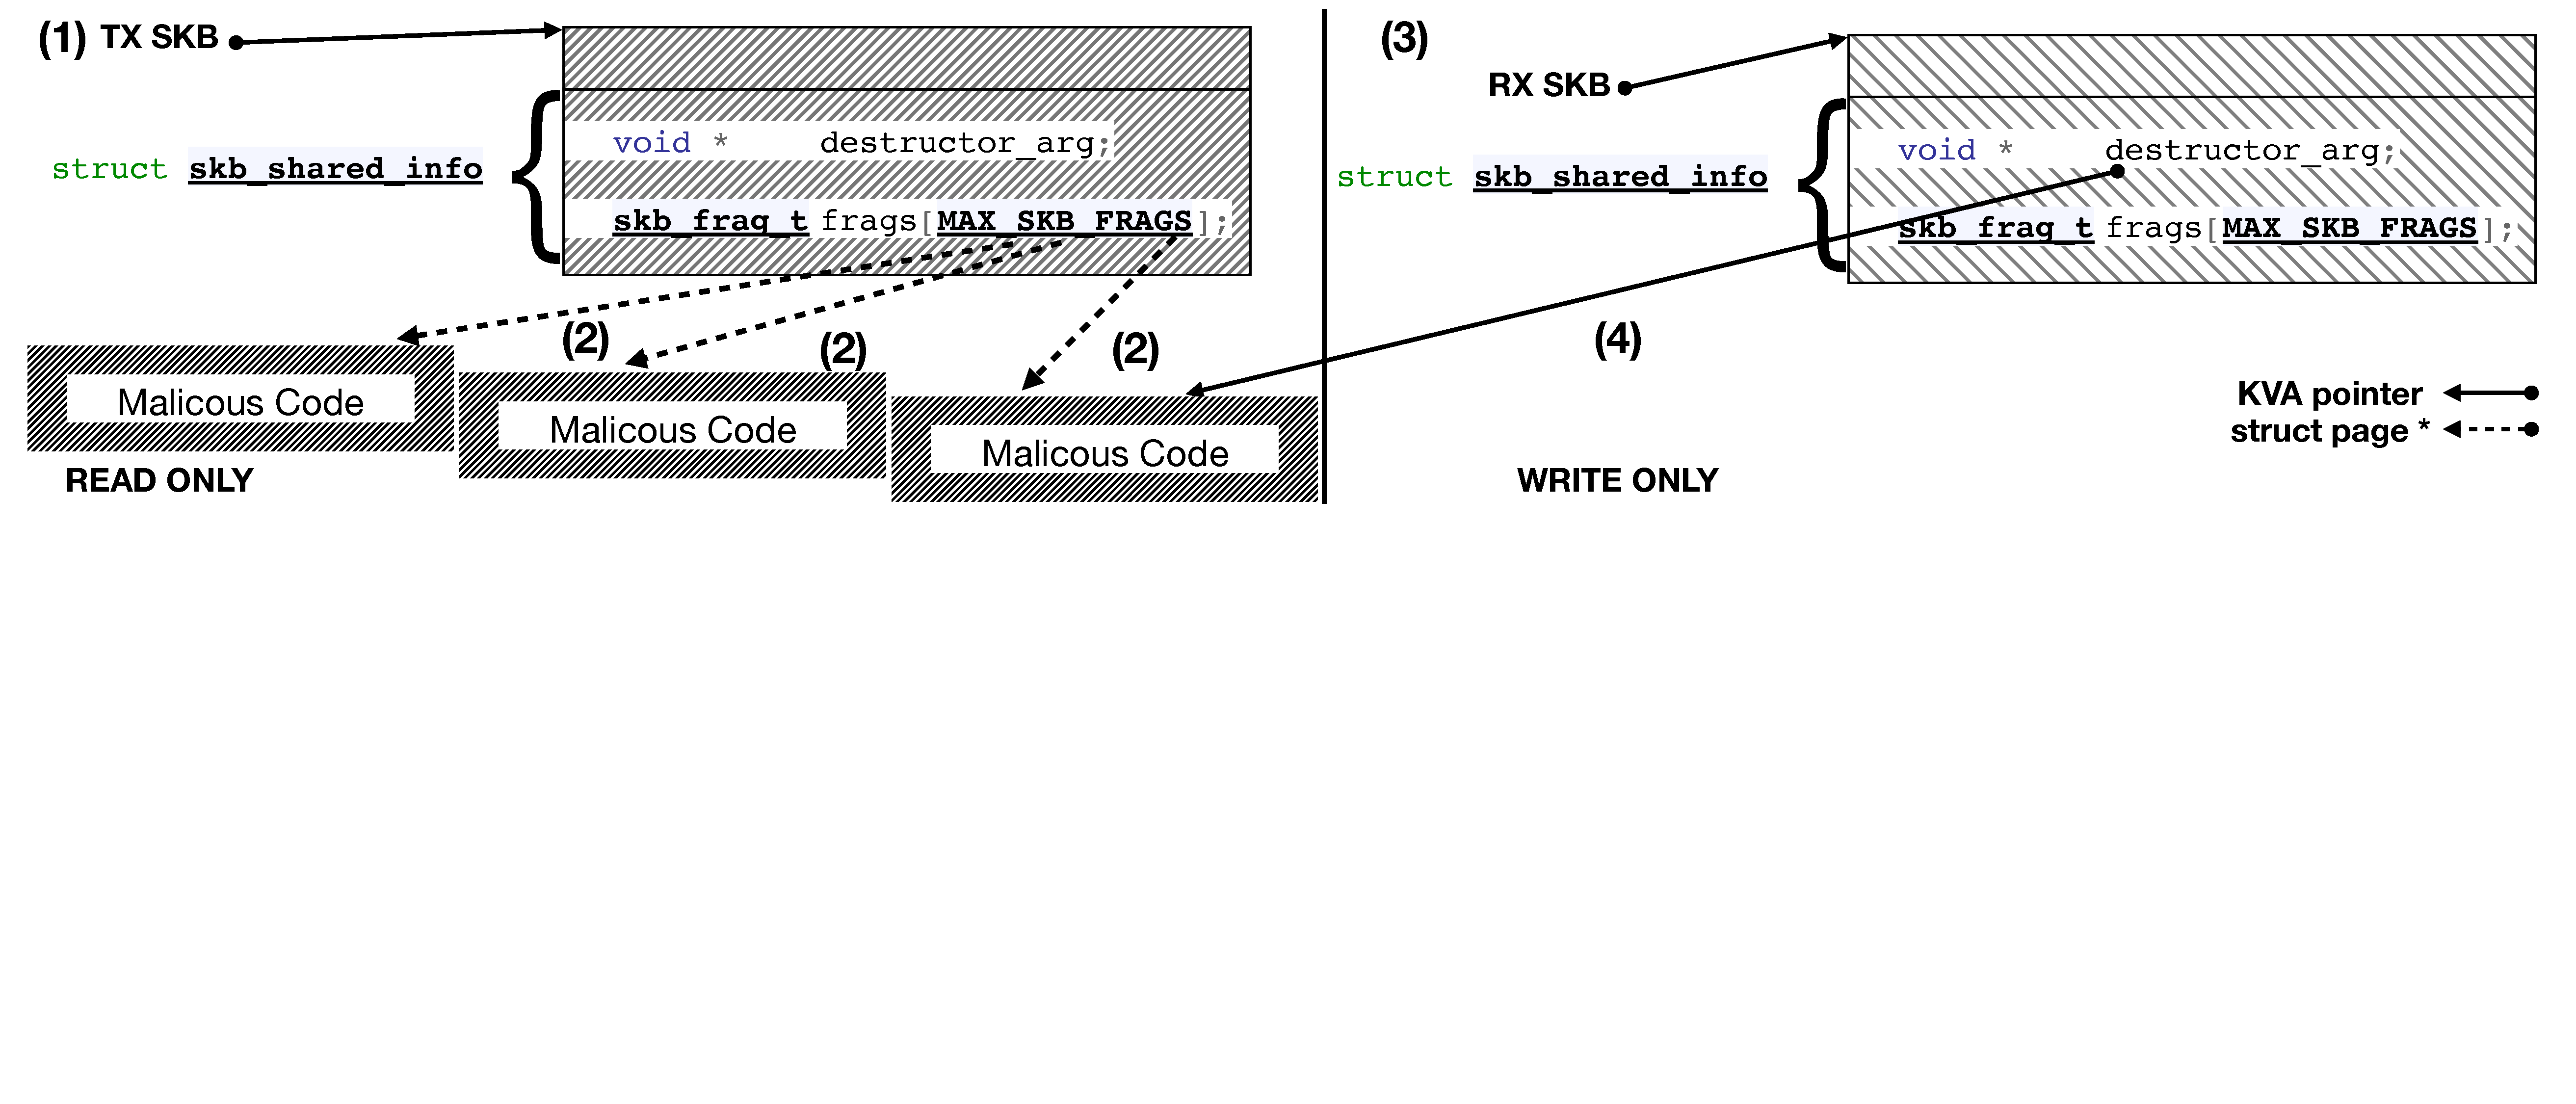
\includegraphics[width=\linewidth]{figs/accomplice.pdf}
    \caption{A TX sk\_buff filled with malicious code, used as a \means for a DMA attack}
    \label{fig:payload}
\end{figure*}
\subsection{Poisoned TX}\label{sec:posion}

\textcolor{magenta}{RingFlod \ref{sec:ringflod} allows a NIC to execute random code with high probability. The prerequisite, is enough information regarding the physical layout of the server and its peripherals\footnote{Other PCIe devices and their location, this all impacts how memory is allocated} and as long as the NIC driver has a high enough memory footprint. }

When guessing a \emph{magic} PFN is not an option, we need other \means of computing a valid \kva. 
A NIC has READ access to the \shinfo of a TX packet, this provides the NIC with access to the frags array. The \texttt{frag} array contains struct \page{} pointers, that both leak kernel pointers that allow to break KASLR, and provide the PFNs of specific pages containing data sent from userspace; pages that device can access with READ. 

Assuming, an unprivileged accomplice(witing or unwitting) can open a UDP/TCP socket in user space; this user could transmit a poisoned ROP buffer. 
%For a ROP attack (where we need the Kernel text offsets) we assume the NIC has spoofed an UDP packet with poisoned content for the accomplice to send. 
Once an accomplice sends the packet the NIC can execute the attack in 4 simple steps (Fig \ref{fig:payload}):
\begin{enumerate}
    \item The TX \data and the fragments are mapped for the NIC to read.
    \item The NIC identifies the poisoned buffer and translates \page to \kva.
    \item The NIC spoofs an RX packet, and delays the completion notification of the TX packets (we don't want the \mabaf to be released prematurely).
    \item The NIC overwrites \shinfo with the \kva retrieved in step 2. 
\end{enumerate}
%But if the fragments hold malicious content; its all the malicious NIC needs for a successful attack. The readable \shinfo holds a \kva for a \page. This both allows the NIC to break KASLR and gives a \kva\footnote{\textcolor{magenta}{Do show exactly what are the KASLR bits and how you break it}} of a valid \mabaf. To implement the attack the NIC will generate an RX packet and fill the \uarg address from the calculated \kva.
%The NIC will hold off on the TX completion event in order to make sure that \kva is not freed by the TX completion handler; before the poisoned RX packet is processed. A TX completion event that fails to appear in due time, will trigger a TX T/O error that will flush all buffers; the T/O is set by the driver usually to 5 seconds, which is enough to implement an attack.\newline
In this scenario the attacker doesn't need any prior knowledge of the kernel or the hardware. The only assumption is that there is an accomplice (witting or unwitting) that can open a socket in user-space. For that matter, a socket in user-space of a guest machine; making any cloud VM or a Proxy server a valid intrusion tool in the presence of a malicious device.\newline
Having an accomplice, in the form of an unprivileged user provides other vectors of attack as well. In addition to running ROP attacks; the NIC can also leak the content of arbitrary memory pages to the user. Assuming that the NIC has write access to \shinfo after it has been sent up the network stack. For example, in case of deferred protection or when pool\_page is used (see \ref{sec:xdp}). The NIC can modify the \page address in the \texttt{frag} entries, and let the Linux network stack copy the context of arbitrary memory pages to an unprivileged user. A likely side effect of this attack is a memory corruption and a Kernel panic; so caution is advised. The reason beaing, that the \texttt{skb\_free} function will attempt to free these pages; pages never owned by the network stack.
\newline
\textcolor{magenta}{Must validate feasibility: An accomplice in user space, can attempt running arbitrary code in kernel context without resolving to ROP attacks; the usef, can instead write a function and a \texttt{ubuf\_info} in an unprivileged binary and send the \texttt{ubuf\_info} address to the NIC. The \shinfo callback must be called with the users page tables loaded - this is a likely scenario as it seems that the \skb is freed inside the recv() sys\_call callback.}

\subsection{Forward Thinking}
In some situations, an accomplice will not be available. Packet forwarding functionality is usually disabled by default in Linux machines. But some Linux servers may function as a router or an L3 load balancer; these machines will have packet forwarding enabled. In this scenario instead of waiting for an accomplice to send a poisoned packet; the NIC can independently generate an RX packet to a destination that is reachable from the server. For a TCP connection, the Linux kernel will attempt to aggregate multiple TCP segments into a single large packet\footnote{Generic Receive offload,\url{https://access.redhat.com/documentation/en-us/red_hat_enterprise_linux/6/html/performance_tuning_guide/network-nic-offloads}}. This packet will then be forwarded and become a TX packet. A TX packet that can be used as described in the previous attack (\ref{sec:posion}) Fig \ref{fig:payload}. \newline
Packet forwarding, also opens up additional attack options. Instead of sending a TCP packet and letting the GRO layer fill in the \texttt{frags} information. The NIC can generate a small UDP packet and fill in the \texttt{frags} array with any arbitrary \page on the system. This will make the driver map these pages with DMA\_TO\_DEVICE; providing read access to any page on the system to the NIC. The ConnectX-5 driver (mlx5\_core), will map all the frags in \shinfo, w/o checking the actual packet length. It is important to set the \texttt{nr\_frags} field to let the driver know that there are frgas to map. But setting the field back to zero, before creating a TX completion. It is important, that the OS wont try freeing pages the driver never owned.

\begin{figure*}[t]
    \centering
    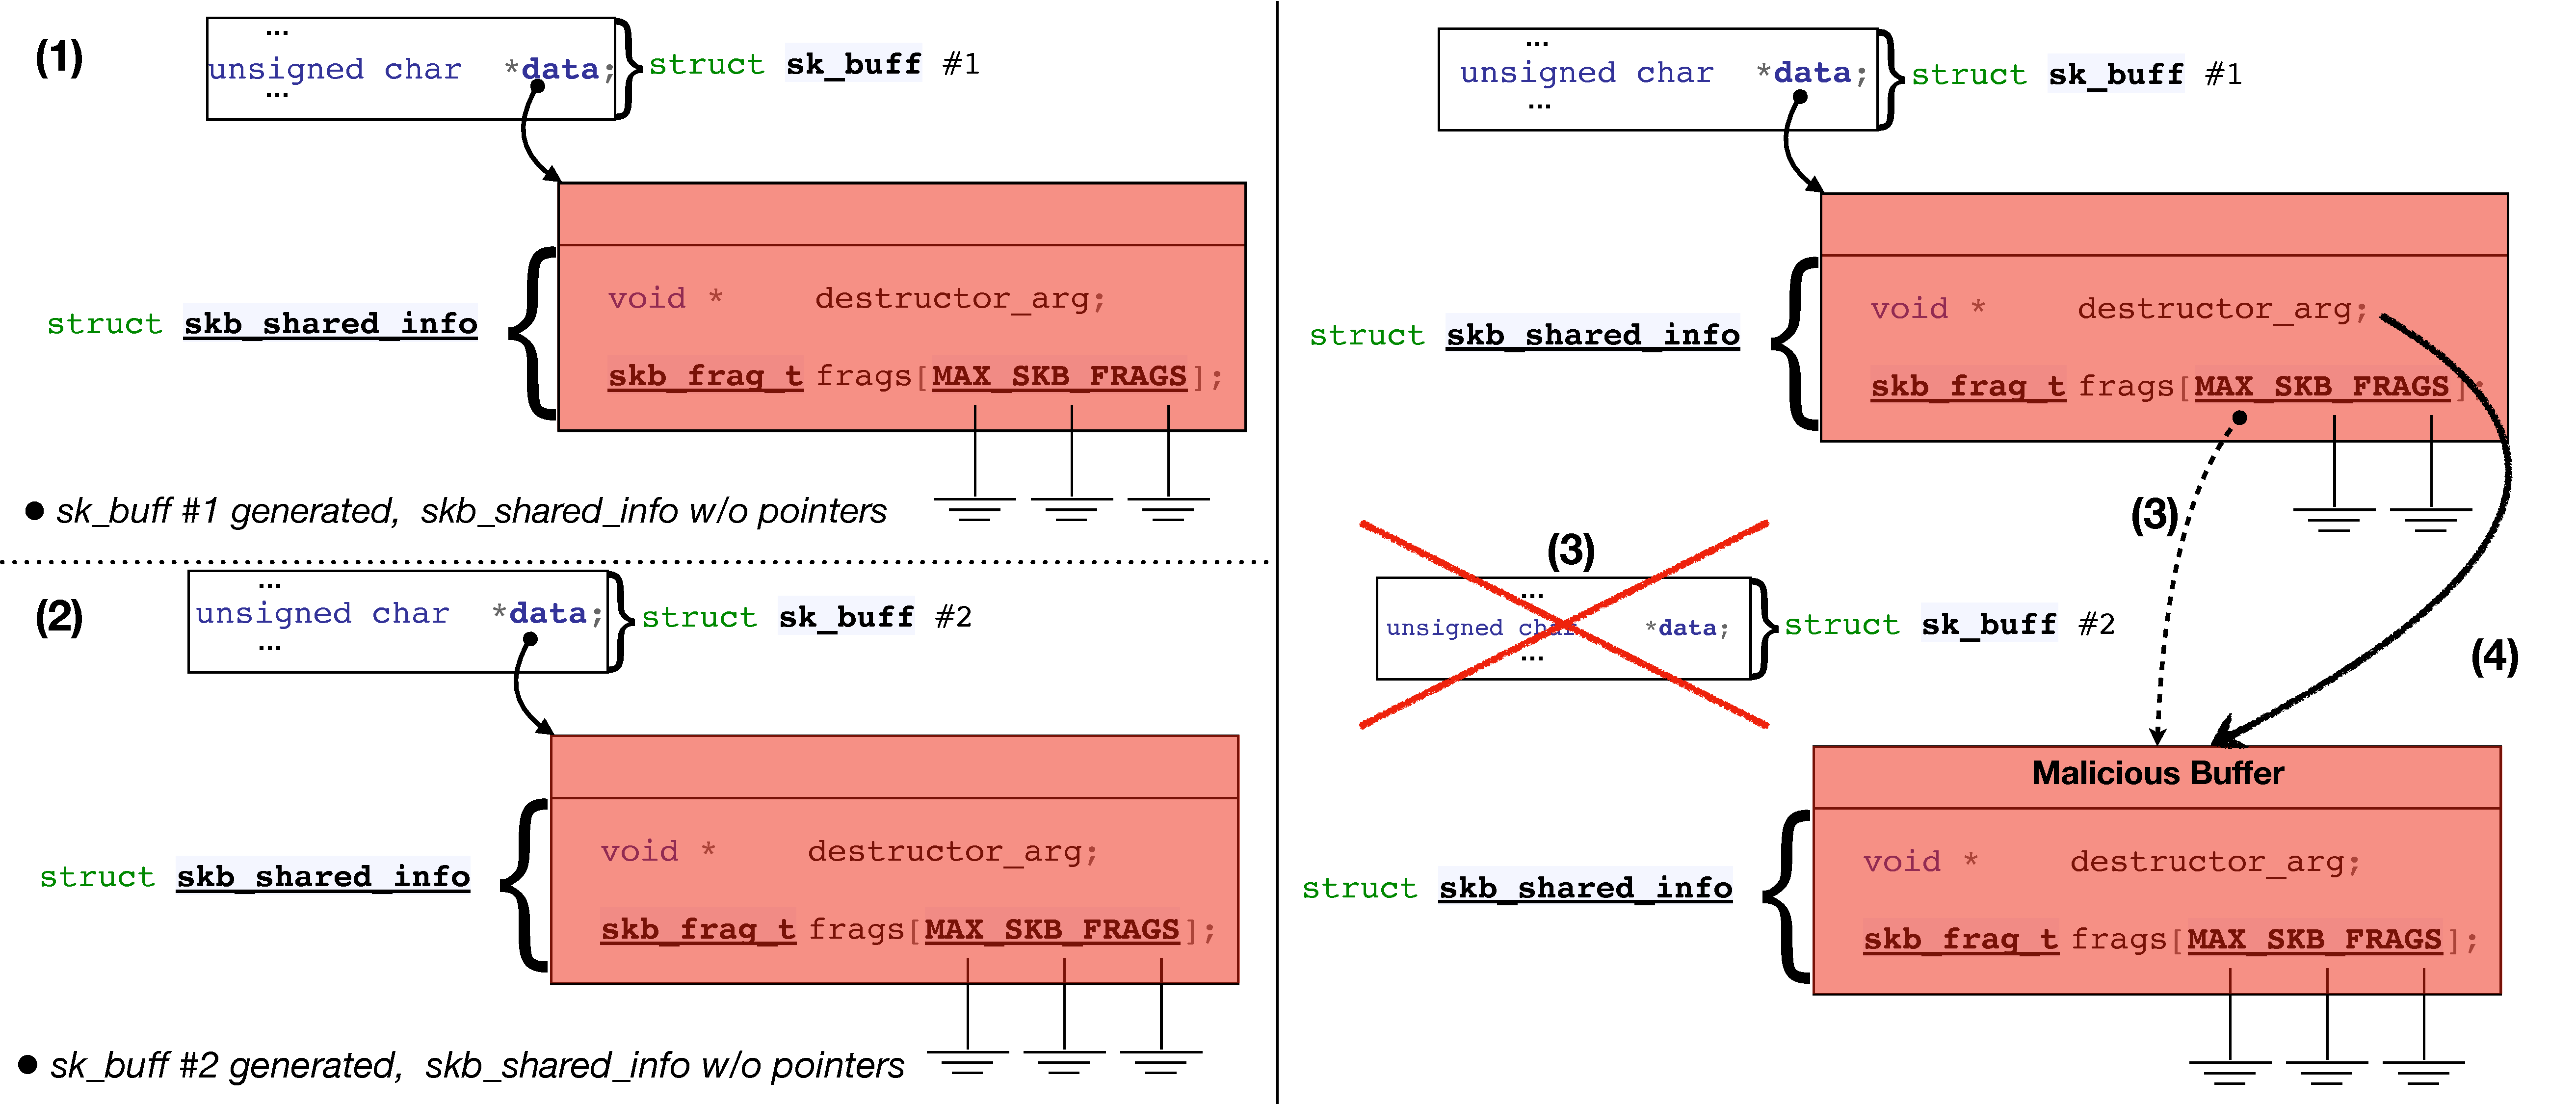
\includegraphics[width=\linewidth]{figs/gro.pdf}
    \caption{An RX sk\_buff after GRO, used as a \means for a DMA attack}
    \label{fig:gro}
\end{figure*}

\subsection{XDP}\label{sec:xdp}
XDP\footnote{\url{https://www.iovisor.org/technology/xdp}} provides a way for users to add custom handling to RX buffers with little overhead. Use cases, include DDOs mitigation for security and Forwarding and load balancing; for the latter the RX buffers need to be also readable to the NIC. As a result all RX buffers are mapped with DMA\_BIDIRECTIONAL rather than the usual DMA\_FROM device. Additionally, in an attempt to avoid performance penalties from memory allocation \cite{xdp} and DMA mapping/unmapping; the RX buffers are reused in a page\_pool\cite{page_pool}. These, pages are never unmapped, and remain accessible to the device both for read and write through out the pools existence (read forever). In this section we will focus on the latest mlx5\_core drivers of the NICs we have on our setup. Other drivers with XDP patches show similar behaviour\footnote{\textcolor{red}{Add a list of drivers to Appendix}}. It is important to note, that a DMA-page pool mechanism is not an inherently bad idea when implemented with caution\cite{MSMT18}. Also, its important to note that the mlx5\_core driver has two modes of operation; linear - where an skb is built around an RX buffer and non-linear where the driver is is filling up the \texttt{frags} of \shinfo. The former is the default, and the later is actually secure. The non-linear mode of option is secure because \shinfo is never accessible to the device; and thus the NIC never has the \oportunity to attack.\newline
In linear mode the NIC has both read, and write access to \shinfo; this additional read capability allows the NIC to run and exploit in 4 steps (Fig \ref{fig:gro}):
\begin{enumerate}
    \item An RX \skb is generated, its part of a TCP stream. \shinfo is initialised by the CPU and the \texttt{frags} are filled with NULL pointers.
    \item A second RX \skb is generated and its part of the same TCP stream.
    \item The second \skb is coalesced with the first packet. The \skb is freed and the \data is added as a \texttt{frag} to the first \skb.
    \item The NIC reads the updated \texttt{frag} field, translates the \page address to a valid \kva and finally fills the \texttt{destructor\_arg} field. Creating a poisoned \skb like in Fig \ref{fig:sh_info}.
\end{enumerate}
The difference between this flow and a regular receive flow is the additional read capability the NIC has due to XDP.
\textcolor{magenta}{\subsection{ICMP}
In the ICMP code I have noticed; what seems to be a reuse of RX skbs for TX, resulting in READ/WRITE mapping - this can allow the device to read all server memory. Unfortunately privilege escalation is infeasible due to lack of \means, until of-course we find a scenario where ICMP adds, write accessible frags.} 

\begin{comment}
%The linear skbs in mlx5 are mapping sh\_info as BI\_DIR, need to see when linear used vs non-linear and to check othe XDP drivers. When sh\_info is mapped BI\_DIR its all we need to attack.\newline It seems linear skb (No (HW?)LRO and MTU<1500 : verify with experimnt or Boris) means no frags, while \begin{enumerate}
%    \item build\_skb is used on a mapped page
%    \item page is unmapped in a deferred way, regardless of iommu policy; a driver hack.
%\end{enumerate} 
 \begin{enumerate}
    \item skb\_try\_coalesce
    \item SW LRO/GRO
\end{enumerate}.
\newline
\textcolor{magenta}{In addition reviewing other drivers for the intersection of DMA\_BIDIR \^ (skb\_add\_rx\_frag||skb\_fill\_page\_descriptor)}
\end{comment}

\textcolor{red}{
\subsection{A Foreigner in a Foreign Land}
Must validate feasibility: An accomplice in user space, can attempt running arbitrary code in kernel context without resolving to ROP attacks; the usef, can instead write a function and a \texttt{ubuf\_info} in an unprivileged binary and send the \texttt{ubuf\_info} address to the NIC. The \shinfo callback must be called with the users page tables loaded - this is a likely scenario as it seems that the \skb is freed inside the recv() sys\_call callback.}


\textcolor{red}{\subsection{ICMP}
In the ICMP code I have noticed; what seems to be a reuse of RX skbs for TX, resulting in READ/WRITE mapping - this can allow the device to read all server memory. Unfortunately privilege escalation is infeasible due to lack of \means, until of-course we find a scenario where ICMP adds, write accessible frags.} 

\begin{comment}
\section{RDMA}
Remote DMA(RDMA)\footnote{Member Companies of Openfabrics alliance are mostly behind these technologies \url{https://www.openfabrics.org/}} is a set of protocols(Infiniband,IWARP,RoCE) that facilitate access to the main memory of a remote machines. We wanted to see if some of the attacks could be perpetrated via a malicious peer.  
We didn't find any risks associated with RDMA, other than the risks associated with device drivers, listed in this paper. The ipoib driver is one such driver, one which also maps \shinfo. A malicious device is still needed, as the post\_send/post\_receive API used by the ipoib driver is similar in function to the usual way NICs function; namely a remote user can't pick where to write or choose to write more than once to the same address. These kinds of operations are supported by rdma\_read/write API; which provides the peer with the ability to read/write from/to a specified addresses. We didn't find any uses for this kind of API in the Linux kernel. With post\_send/post\_receive API, the remote host can only modify legitimate memory buffers; and thus can't take advantage of sub-page vulnerabilities.
\textcolor{red}{Am I answering a question that no one asked?}
%\textcolor{red}{AFAIK; besides Linux only Windows supports RDMA in the kernel}
\end{comment}

\section{Related work}

%\subsection{Circumventing IOMMU}

%The IOMMU is open to several new kinds of attacks whose goal is to eliminate its protection. The first type target bad IOMMU implementations and the second focus on wrong initialization of the IOMMU. An example of bad implementations is the lack of interrupts remapping in the first IOMMU versions. Without the ability to forward only legitimate interrupts to the correct virtual machine, malicious devices might also generate on the host other interrupts. Rutkowska and Wojtczuk attacked the Intel VT-d by creating fake interrupts at the host, successfully executing code thanks to a bug in the interrupt mechanism on Intel machines \cite{WR11}. An example of wrong initialization is enabling I/O devices before setting up the IOMMU. Morgan et al. attacked the IOMMU by overriding its tables during initialization \cite{MANK16}. 
%Frisk used a similar approach for stealing Apple FireVault passwords \cite{Cim16}. Sang et al. used both methods for several attacks \cite{SLND10}. First, they exploited the ability of the Intel VT-d to reduce IOTLB overhead by distributing entries to compatible I/O devices. Using this ability, malicious I/O devices can report false entries in order to access protected memory areas. Second, they capitalized on the fact that old implementations of the IOMMU identified I/O devices by self declarations. Malicious I/O devices can spoof the ID of an innocent one in order to access its memory. Last, they demonstrated how malicious I/O devices might exploit memory sharing with other I/O devices. Such sharing could, for example, be a decision of the OS according to the hardware topology. The picture would not be complete without an overview of attacks that simply ignore the presence of the IOMMU. 

%Also, modern IOMMU/PCI architectures includes the address translation services feature (PCI ATS; aka Device-IOTLB) that allows peripheral devices to serve as their own IOTLB. This feature is very unsecure and, in fact, lets malicious devices bypass the IOMMU protection by providing fake translations. In this work, we assume that the IOMMU is working as expected, so that it is possible to write an OS from scratch that utilizes the IOMMU correctly. OSs, however, are rarely written from scratch, as doing so is a very complex task. Our attacks thus target the methodology used by all commodity OSs to utilize the IOMMU in the real world. We have ignored ATS as it is unsecure by design.
%\end{comment}

%\subsection{Protecting Against New attacks}
%Deferred mode vulnerability could be mitigated by simply stopping batch IOTLB invalidations.
%To reduce performance overheads, one may batch the entire unmapping process rather than only the invalidation. Implementing such a solution will require a new memory management mechanism to keep the pages owned by the device. Implementing a page ownership mechanism could be beneficial for other cases as well, such as zero-copy buffers—which may be owned by one of the device, the kernel and user-level applications.

%Sub-page vulnerability results from the gap between hardware design and software usages. Hence, it could be mitigated by modifying either the software or the hardware. Software modifications could be done either by repairing all broken drivers or, preferably, by changing the DMA layer so that it becomes aware of the size discrepancy. Hardware modification must be done centrally in the IOMMU in order to support legacy devices. Any solution that requires changes in I/O devices implies that secured environments could not include any currently existing device. In addition, common techniques against heap-overflow vulnerabilities might be used for making the attacks harder even though they will not completely eliminate them, as demonstrated above.
%One possible software solution is to repair each and every driver that uses DMA. By making sure that drivers allocate memory for devices only in a page granularity, one could eliminate all sub-page issues. Even though this is probably the most obvious solution, it has the disadvantage of requiring a big change in existing code. In particular, legacy unsupported drivers must also be fixed to ensure that the system is truly secured. In addition, since every new driver should follow this guideline, the chance of creating new bugs is very high. This latter issue could be solved by additionally changing the DMA interface to accept only whole page mapping rather than arbitrary sized buffers.


Currently, several hardware mechanisms exist for protecting CPU buffers smaller than a page. These mechanisms could be implemented in the IOMMU in order to mitigate the sub-page granularity vulnerability. Intel’s sup-page protecting technology suggests protecting fixed sized buffers smaller than a page \cite{Int18}. Since the buffers are still fixed sized, the same vulnerability remains, albeit in a more limited way. Intel MPX (Memory Protection Extensions) lets the user define boundaries for buffers and, later, explicitly checks that the corresponding pointers are between these boundaries \cite{Int16a}. Oracle SSM (Silicon Secured Memory) lets the user “color” buffers and associative pointers \cite{Ora15}. The color is implicitly checked for a match at each memory access. MPX, SSM and other similar approaches may be used for building a secure alternative for IOMMU. 

%In practice, this means that the mappings are arbitrarily sized. An example of such an alternative is rIOMMU, which was designed to work optimally with network cards \cite{MABYT15}.

%Standard memory protection mechanisms include restriction of code executing areas and memory encryption. As we have shown above, DEP/kASLR do not prevent sub-page attacks. Encrypting sensitive data could prevent some forms of attacks (e.g., immediate data leakage). By leaking data using code that was injected by the DMA, Blass et al. have shown that encrypting sensitive data is not enough \cite{BR12}.

Common techniques against heap-overflow vulnerabilities may also be useful when they are properly implemented. 

%For example, a recent Linux kernel patch suggests obfuscating the SLUB freelist by xor-ing its pointers with a random value \cite{Coo17}. This technique is very helpful in the case of simple heap overflow. In our scenario, however, the device was often able to read writable pages. Furthermore, old IOMMUs without special support of zero-length reads require writable pages to be readable as well \cite{Int16b}. Since the device can read the entire page, it is possible to deduce the random value from multiple obfuscated pointers. In contrast, obfuscating a single sensitive pointer poses a real difficulty to the exploiter even if the obfuscated pointer could be read first.
%A completely different approach is to try to reduce the damage a working attack might cause rather than preventing it completely. This could be done by monitoring the behavior of devices and drivers for potential dangers. As with classic DMA attacks, monitoring the bus activity, looking for anomalies in DMA activity might be helpful for detecting live attacks \cite{Ste13}. This technique, however, still requires modeling each device DMA activity \cite{Ste14}. Similarly, monitoring mapping requests could be helpful during development. For example, one may look for known patterns, such as pointers or passwords, in a page during its mapping and detect bad practices in time.

 
\textcolor{magenta}{Need to mention new (Non default - Only impacts RingFlod)kernel configs SHUFFLE\_PAGE\_ALLOCATOR \url{https://lore.kernel.org/patchwork/patch/1037734/}}







%%%%%%%%%%%%%%%%%%%%%%%%%
%%%%%%%%%%%%%%%%%%%%%%%%%

Naturally, preventing DMA attacks is also of interest in academic research. Proposed solutions include storing secret data in the CPU registers to prevent the data from being leaked \cite{MFD11, CZG15, Sim11} and monitoring the bus activity using hardware performance counters and finding anomalies in DMA activity \cite{Ste13}. However, the former does not prevent the devices from modifying the OS memory \cite{BR12}, whereas the latter requires modeling each device’s DMA activity \cite{Ste14}, which is arguably unreasonable.




\section{Conclusion}

Hardware attacks are often considered to be harder to implement than software attacks. Nevertheless, once a malicious device is built, launching the attack is as easy as connecting the device to an external port for only a few seconds. Recent leaks from clandestine agencies show that they attacked both by shipping infected hardware \cite{Gal14} and by connecting external malicious devices \cite{Fin14}. Hence, the problems really do exist in the wild and should concern security experts. Moreover, our FireWire/SPB2 attack can be seen as an expansion of the classic attacks and could easily be added as a module to existing off-the-shelf attacking tools.
The main limitation of our attacks compared to the old ones is that the devices in our attacks have access only to part of the memory. For instance, memory dumping, a popular DMA attack, has become much less trivial thanks to the IOMMU. In the extreme case, the attacker has access only to one page without even knowing its physical address. As a result, our attacks had to be made more complicated than the old ones. For example, code injection might be required for memory dumping, and payload spraying for overcoming unknown physical addresses.
Generally speaking, the requirement for physical access means that the attacks are targeted albeit this need not be true. There are some methods for spreading opportunistic attacks using physical devices. In some case, modifying firmware to be malicious could be done entirely by software that, in its turn, could be distributed over the network (e.g., Bad USB attack \cite{NL14}). In some cases, the attack could even come from the network side of the device [Ben17a, Ben17b]. Another method is to drop malicious devices in public spaces and wait for a potential victim to connect it to his computer \cite{TDF16}. It is also possible to create a malicious device that can impersonate a legitimate device \cite{thunder}.\newline
While working on the attacks, we realized that the root cause of all the discussed problems comes from the way modern OSs treat peripheral devices. Today, the security industry no longer trusts I/O devices. Recommendations for building trusted environments often include putting limitations on devices, such as removing potentially dangerous drivers or using IOMMU. All state-of-the-art OSs, however, were designed a long time ago. Indeed, when it comes to security, OSs do not treat devices as untrusted entities as they do processes. All the lessons that were learned about protection from/of processes do not seem to have carried over. As a result:
\begin{enumerate}
    \item Memory that is given to the device is not zeroed.
    \item Allocation granularity is not page aligned.
    \item IOTLB invalidations are often deferred.
    \item IOVAs are not randomized and are predictable. \textcolor{red}{What? How are they predictable, and how does it help?}
    \item There are no checkers for invalid memory use (such as Linux’s KASAN for regular memory usages)
\end{enumerate}
Even though we explored only some aspects of this problem, this is a fundamental design issue and it should be addressed as such. Finally, we note that current IOMMU/PCI architectures allow peripheral devices to serve as their own IOTLB (namely, PCI ATS or Device-IOTLB). This technology makes our work meaningless because, by using it, malicious devices are able to simply report false translations and access any protected memory\footnote{It is now possible to disable ATS functionality with a boot parameter}.

\begin{comment}
\footnote{\url{https://lore.kernel.org/lkml/20180510230948.GF190385@bhelgaas-glaptop.roam.corp.google.com/}}.
\end{comment}

%To somewhat enhance the security of Linux, we suggested a patch allowing system administrators to disable ATS.1 Development of this patch continues and it will most likely be introduced by Linux into one of its upcoming versions.\newline
%DMA attacks are feasible and should not be treated lightly. IOMMU subverting attacks are avoidable, but none of the solutions can be found in the wild. Better kASLR, NX-BIT and better API are all needed to prevent IOMMU subverting techniques. 
Its important to note, that no DMA attack could work without sub-page vulnerability; the unintentional exposure of restricted fields. Working on the various attacks, we have noticed that, with the existing API used for I/O operations it is very difficult not to create a sub-page vulnerability. The \textit{dma\_map\_single} call asks the caller for a pointer and a length; this API insinuates that only the mapped bytes will be exposed; we know this to be untrue. The \textit{dma\_unmap\_single}, insinuates that the buffer will not be accessible to the device after the call; this is also untrue, both due to deferred protection and sub-page vulnerabilities. To a lesser degree, the \textit{build\_skb} is also dangerous. This call allows building an \skb around an arbitrary buffer. This is dangerous, because this seems to encourage building an \skb around a dma mapped buffer; exposing \shinfo. In fact, we were looking for this function when working on a list of vulnerable device drivers. We contend, that a better API would lead to a better code. Using the staunch, \textit{dma\_\{un\}map\_page} or using tools like \textit{dma\_page\_pool}. \textcolor{magenta}{Or even complete solutions not unlike what was proposed in DAMN\cite{MSMT18,MMT16}; - To much?} provides the driver authors with better options for writing secure and performant drivers. 

%\subsection{Mitigations in the wild}
%\textcolor{magenta}{I imagine a table with OS on Y and best practices on X. IOMMU policy, KASLR, NX-bit, discriminate mapping (R or W, not both), device IOVA separation, sand boxing mapped addresses. Kernels Win,MacOS,FreeBSD - use NDSS paper, contribution: ESX (Need to send some emails), Linux - Ubuntu versions, Sless?(RHEL)}.


\textcolor{blue}{
Our actionable conclusions:
\begin{enumerate}
    \item Static code analysis for DMA vulnerabilities.
    \item Remove DMA Mapping API, adopt DAMN instead. \label{act:damn}
    \item Remove mixed linear/non-linear skbs, add checks into \shinfo API.
    \item Better API is needed for I/O operations
    \begin{itemize}
        \item I/O buffer creation, discourage bad habits (build\_skb).
        \item Remove dma\_map\_single (Or adopt \ref{act:damn})
        \item Better memory allocation - namely I/O buffers like page\_frag, page\_pool or DAMN.
    \end{itemize}
\end{enumerate}
\texttt{All DMA attacks steam from this vulnerability.}
}

It is important to note, that a DMA-page pool mechanism is not an inherently bad idea when implemented with caution\cite{MSMT18}. 

%\section{Appendix A}

\subsection{All contributions made in Gils work \cite{gil}}

\begin{description}
  
\item[Sub Page] Exploiting the sub page vulnerability to access metadata.
\item[Deferred protection] Exploiting IOTLB invalidation to hack correct NIC drivers.
\item[KASLR] Reading random ptrs to guess the random address bits, Leaking data via Sub Page.
\item[FreeBSD UMA] Hacking FreeBSD memory allocator.
\item[\texttt{Question RDMA}] Can IPoIB driver be exploited in additional ways? Other RDMA issues.
\end{description}

\subsection{All contributions made in NDSS paper\cite{thunder}:}
\begin{description}
\item[attack 1,2] Windows attacks, irrelevant.
\item[attack 3] MAC OS reading VPN data, irrelevant.
\item[attack 4] Shared mappings between devices: MAC OS (Also Windows)mbufs open to read/write - Same as Gils  attack \#1 on thunderbolt.
\item[attack 5] FreeBSD per device iommu:  Same as Gils  attack \#1 on thunderbolt (p.9). Mention that Linux is invulnerable.
\item[attack 6] Linux leaks nat tables - random subpage hits - No known IOVA, NO way of knowing as READ=!Write
\item[attack 7] Linux leaking data by avoiding TX completions - would hit T/O issues and driver restart.
\item[attack 8] ATS - Self serve IOMMU by NIC. 
\end{description}

\subsection{Shared contributions:}
\begin{description}
\item[Sub Page] Shared Mdata - Data mapping.
\item[KALSR] KASLR leaking due to sub page.
\end{description}

\subsection{New Contribution}

\begin{description}
\item[skb shared info] Shared Mdata in Linux skb. 
\item[page cahe colocation] RX data allocated from page cache - means that after unmap page is still accessible via iova of next buffer - (strict and deferred vulnerable). This is stronger then sub page, as dense mappings 
allow for an attack even with strict API and correct ordering.
\item[RingFlod] Determining PFNs for attack. \texttt{What else is accessible by the NIC, what config, FW return codes/values? - Is kva visible}.
\item[HOTPage] A TX page reused in RX - allowing for temp R/W access with open valid kva (zero knowledge)-- \texttt{I'm pretty sure overlap is impossible and this approach is invalid}.
\end{description}

\bibliographystyle{plain}
\bibliography{references}

%%%%%%%%%%%%%%%%%%%%%%%%%%%%%%%%%%%%%%%%%%%%%%%%%%%%%%%%%%%%%%%%%%%%%%%%%%%%%%%%
\end{document}
%%%%%%%%%%%%%%%%%%%%%%%%%%%%%%%%%%%%%%%%%%%%%%%%%%%%%%%%%%%%%%%%%%%%%%%%%%%%%%%%
